% !TeX spellcheck = pl_PL
%%%%%%%%%%%%%%%%%%%%%%%%%%%%%%%%%%%%%%%%%%%
%                                        %
% Szablon pracy dyplomowej inzynierskiej %
% zgodny  z aktualnymi  przepisami  SZJK %
%                                        %
%%%%%%%%%%%%%%%%%%%%%%%%%%%%%%%%%%%%%%%%%%
%                                        %
%  (c) Krzysztof Simiński, 2018-2023     %
%                                        %
%%%%%%%%%%%%%%%%%%%%%%%%%%%%%%%%%%%%%%%%%%
%                                        %
% Najnowsza wersja szablonów jest        %
% podstępna pod adresem                  %
% github.com/ksiminski/polsl-aei-theses  %
%                                        %
%%%%%%%%%%%%%%%%%%%%%%%%%%%%%%%%%%%%%%%%%%
%
%
% Projekt LaTeXowy zapewnia odpowiednie formatowanie pracy,
% zgodnie z wymaganiami Systemu zapewniania jakości kształcenia.
% Proszę nie zmieniać ustawień formatowania (np. fontu,
% marginesów, wytłuszczeń, kursywy itd. ).
%
% Projekt można kompilować na kilka sposobów.
%
% 1. kompilacja pdfLaTeX
%
% pdflatex main
% bibtex   main
% pdflatex main
% pdflatex main
%
%
% 2. kompilacja XeLaTeX
%
% Kompilatacja przy użyciu XeLaTeXa różni się tym, że na stronie
% tytułowej używany jest font Calibri. Wymaga to jego uprzedniego
% zainstalowania.
%
% xelatex main
% bibtex  main
% xelatex main
% xelatex main
%
%
%%%%%%%%%%%%%%%%%%%%%%%%%%%%%%%%%%%%%%%%%%%%%%%%%%%%%
% W przypadku pytań, uwag, proszę pisać na adres:   %
%      krzysztof.siminski(małpa)polsl.pl            %
%%%%%%%%%%%%%%%%%%%%%%%%%%%%%%%%%%%%%%%%%%%%%%%%%%%%%
%
% Chcemy ulepszać szablony LaTeXowe prac dyplomowych.
% Wypełniając ankietę spod poniższego adresu pomogą
% Państwo nam to zrobić. Ankieta jest całkowicie
% anonimowa. Dziękujemy!


% https://docs.google.com/forms/d/e/1FAIpQLScyllVxNKzKFHfILDfdbwC-jvT8YL0RSTFs-s27UGw9CKn-fQ/viewform?usp=sf_link
%
%%%%%%%%%%%%%%%%%%%%%%%%%%%%%%%%%%%%%%%%%%%%%%%%%%%%%%%%%%%%%%%%%%%%%%%%%

%%%%%%%%%%%%%%%%%%%%%%%%%%%%%%%%%%%%%%%%%%%%%%%
%                                             %
% PERSONALIZACJA PRACY – DANE PRACY           %
%                                             %
%%%%%%%%%%%%%%%%%%%%%%%%%%%%%%%%%%%%%%%%%%%%%%%

% Proszę wpisać swoje dane w poniższych definicjach.

% TODO
% dane autora
\newcommand{\FirstNameAuthor}{Jakub}
\newcommand{\SurnameAuthor}{Ciołek}
\newcommand{\IdAuthor}{295618}   % numer albumu  (bez $\langle$ i $\rangle$)

% drugi autor:
%\newcommand{\FirstNameCoauthor}{Imię}   % Jeżeli jest drugi autor, to tutaj należy podać imię.
%\newcommand{\SurnameCoauthor}{Nazwisko} % Jeżeli jest drugi autor, to tutaj należy podać nazwisko.
%\newcommand{\IdCoauthor}{$\langle$wpisać właściwy$\rangle$}  % numer albumu drugiego autora (bez $\langle$ i $\rangle$)
% Gdy nie ma drugiego autora, należy zostawić poniższe definicje puste, jak poniżej. Gdy jest drugi autor, należy zakomentować te linie.
\newcommand{\FirstNameCoauthor}{} % Jeżeli praca ma tylko jednego autora, to dane drugiego autora zostają puste.
\newcommand{\SurnameCoauthor}{}   % Jeżeli praca ma tylko jednego autora, to dane drugiego autora zostają puste.
\newcommand{\IdCoauthor}{}  % Jeżeli praca ma tylko jednego autora, to dane drugiego autora zostają puste.
%%%%%%%%%%

\newcommand{\Supervisor}{Dr inż. Ewa Płuciennik}     % dane promotora (bez $\langle$ i $\rangle$)
\newcommand{\Title}{Aplikacja do symulacji rozprzestrzeniania się zarażeń}           % tytuł pracy po polsku
\newcommand{\TitleAlt}{Application for simulating the spread of infections.}                     % thesis title in English
\newcommand{\Program}{Infromatyka}            % kierunek studiów  (bez $\langle$ i $\rangle$)
\newcommand{\Specialisation}{Bazy danych i Inżynieria Systemów}     % specjalność  (bez $\langle$ i $\rangle$)
\newcommand{\Departament}{Informatyki Stosowanej}        % katedra promotora  (bez $\langle$ i $\rangle$)

% Jeżeli został wyznaczony promotor pomocniczy lub opiekun, proszę go/ją wpisać ...
\newcommand{\Consultant}{} % brak promotowa pomocniczego / opiekuna

% koniec fragmentu do modyfikacji
%%%%%%%%%%%%%%%%%%%%%%%%%%%%%%%%%%%%%%%%%%


%%%%%%%%%%%%%%%%%%%%%%%%%%%%%%%%%%%%%%%%%%%%%%%
%                                             %
% KONIEC PERSONALIZACJI PRACY                 %
%                                             %
%%%%%%%%%%%%%%%%%%%%%%%%%%%%%%%%%%%%%%%%%%%%%%%

%%%%%%%%%%%%%%%%%%%%%%%%%%%%%%%%%%%%%%%%


%%%%%%%%%%%%%%%%%%%%%%%%%%%%%%%%%%%%%%%%%%%%%%%
%                                             %
% PROSZĘ NIE MODYFIKOWAĆ PONIŻSZYCH USTAWIEŃ! %
%                                             %
%%%%%%%%%%%%%%%%%%%%%%%%%%%%%%%%%%%%%%%%%%%%%%%



\documentclass[a4paper,twoside,12pt]{book}
\usepackage[utf8]{inputenc}                                      
\usepackage[T1]{fontenc}  
\usepackage{amsmath,amsfonts,amssymb,amsthm}
\usepackage[british,polish]{babel} 
\usepackage{indentfirst}
\usepackage{xurl}
\usepackage{xstring}
\usepackage{ifthen}



\usepackage{ifxetex}

\ifxetex
\usepackage{fontspec}
\defaultfontfeatures{Mapping=tex—text} % to support TeX conventions like ``——-''
\usepackage{xunicode} % Unicode support for LaTeX character names (accents, European chars, etc)
\usepackage{xltxtra} % Extra customizations for XeLaTeX
\else
\usepackage{lmodern}
\fi



\usepackage[margin=2.5cm]{geometry}
\usepackage{graphicx} 
\usepackage{hyperref}
\usepackage{booktabs}
\usepackage{tikz}
\usepackage{pgfplots}
\usepackage{mathtools}
\usepackage{geometry}
\usepackage{subcaption}   % subfigures
\usepackage[page]{appendix} % toc,
\renewcommand{\appendixtocname}{Dodatki}
\renewcommand{\appendixpagename}{Dodatki}
\renewcommand{\appendixname}{Dodatek}

\usepackage{csquotes}
\usepackage[natbib=true,backend=bibtex,maxbibnames=99]{biblatex}  % kompilacja bibliografii BibTeXem
%\usepackage[natbib=true,backend=biber,maxbibnames=99]{biblatex}  % kompilacja bibliografii Biberem
\bibliography{biblio/biblio}

\usepackage{ifmtarg}   % empty commands  

\usepackage{setspace}
\onehalfspacing


\frenchspacing

%%%%%%%%%%%%%%%%%%%%%%%%%%%%%%%%%%
% środowiska dla definicji, twierdzenia, przykładu
\usepackage{amsthm}

\newtheorem{Definition}{Definicja}
\newtheorem{Example}{Przykład}
\newtheorem{Theorem}{Twierdzenie}
%%%%%%%%%%%%%%%%%%%%%%%%%%%%%%%%%%

%%%% TODO LIST GENERATOR %%%%%%%%%

\usepackage{color}
\definecolor{brickred}      {cmyk}{0   , 0.89, 0.94, 0.28}

\makeatletter \newcommand \kslistofremarks{\section*{Uwagi} \@starttoc{rks}}
\newcommand\l@uwagas[2]
{\par\noindent \textbf{#2:} %\parbox{10cm}
	{#1}\par} \makeatother


\newcommand{\ksremark}[1]{%
	{%\marginpar{\textdbend}
		{\color{brickred}{[#1]}}}%
	\addcontentsline{rks}{uwagas}{\protect{#1}}%
}

\newcommand{\comma}{\ksremark{przecinek}}
\newcommand{\nocomma}{\ksremark{bez przecinka}}
\newcommand{\styl}{\ksremark{styl}}
\newcommand{\ortografia}{\ksremark{ortografia}}
\newcommand{\fleksja}{\ksremark{fleksja}}
\newcommand{\pauza}{\ksremark{pauza `--', nie dywiz `-'}}
\newcommand{\kolokwializm}{\ksremark{kolokwializm}}
\newcommand{\cudzyslowy}{\ksremark{,,polskie cudzysłowy''}}

%%%%%%%%%%%%%% END OF TODO LIST GENERATOR %%%%%%%%%%%

\newcommand{\printCoauthor}{%		
	\StrLen{\FirstNameCoauthor}[\FNCoALen]
	\ifthenelse{\FNCoALen > 0}%
	{%
		{\large\bfseries\Coauthor\par}
		
		{\normalsize\bfseries \LeftId: \IdCoauthor\par}
	}%
	{}
} 

%%%%%%%%%%%%%%%%%%%%%
\newcommand{\autor}{%		
	\StrLen{\FirstNameCoauthor}[\FNCoALenXX]
	\ifthenelse{\FNCoALenXX > 0}%
	{\FirstNameAuthor\ \SurnameAuthor, \FirstNameCoauthor\ \SurnameCoauthor}%
	{\FirstNameAuthor\ \SurnameAuthor}%
}
%%%%%%%%%%%%%%%%%%%%%

\StrLen{\FirstNameCoauthor}[\FNCoALen]
\ifthenelse{\FNCoALen > 0}%
{%
	\author{\FirstNameAuthor\ \SurnameAuthor, \FirstNameCoauthor\ \SurnameCoauthor}
}%
{%
	\author{\FirstNameAuthor\ \SurnameAuthor}
}%

%%%%%%%%%%%% ZYWA PAGINA %%%%%%%%%%%%%%%
% brak kapitalizacji zywej paginy
\usepackage{fancyhdr}
\pagestyle{fancy}
\fancyhf{}
\fancyhead[LO]{\nouppercase{\it\rightmark}}
\fancyhead[RE]{\nouppercase{\it\leftmark}}
\fancyhead[LE,RO]{\it\thepage}


\fancypagestyle{tylkoNumeryStron}{%
	\fancyhf{} 
	\fancyhead[LE,RO]{\it\thepage}
}

\fancypagestyle{bezNumeracji}{%
	\fancyhf{} 
	\fancyhead[LE,RO]{}
}


\fancypagestyle{NumeryStronNazwyRozdzialow}{%
	\fancyhf{} 
	\fancyhead[LE]{\nouppercase{\autor}}
	\fancyhead[RO]{\nouppercase{\leftmark}} 
	\fancyfoot[CE, CO]{\thepage}
}


%%%%%%%%%%%%% OBCE WTRETY  
\newcommand{\obcy}[1]{\emph{#1}}
\newcommand{\english}[1]{{\selectlanguage{british}\obcy{#1}}}
%%%%%%%%%%%%%%%%%%%%%%%%%%%%%

% polskie oznaczenia funkcji matematycznych
\renewcommand{\tan}{\operatorname {tg}}
\renewcommand{\log}{\operatorname {lg}}

% jeszcze jakies drobiazgi

\newcounter{stronyPozaNumeracja}

%%%%%%%%%%%%%%%%%%%%%%%%%%% 
\newcommand{\printOpiekun}[1]{%		
	
	\StrLen{\Consultant}[\mystringlen]
	\ifthenelse{\mystringlen > 0}%
	{%
		{\large{\bfseries OPIEKUN, PROMOTOR POMOCNICZY}\par}
		
		{\large{\bfseries \Consultant}\par}
	}%
	{}
} 
%
%%%%%%%%%%%%%%%%%%%%%%%%%%%%%%%%%%%%%%%%%%%%%%

% Proszę nie modyfikować poniższych definicji!
\newcommand{\Author}{\FirstNameAuthor\ \MakeUppercase{\SurnameAuthor}} 
\newcommand{\Coauthor}{\FirstNameCoauthor\ \MakeUppercase{\SurnameCoauthor}}
\newcommand{\Type}{PROJEKT INŻYNIERSKI}
\newcommand{\Faculty}{Wydział Automatyki, Elektroniki i Informatyki} 
\newcommand{\Polsl}{Politechnika Śląska}
\newcommand{\Logo}{graf/politechnika_sl_logo_bw_pion_pl.pdf}
\newcommand{\LeftId}{Nr albumu}
\newcommand{\LeftProgram}{Kierunek}
\newcommand{\LeftSpecialisation}{Specjalność}
\newcommand{\LeftSUPERVISOR}{PROWADZĄCY PRACĘ}
\newcommand{\LeftDEPARTMENT}{KATEDRA}
%%%%%%%%%%%%%%%%%%%%%%%%%%%%%%%%%%%%%%%%%%%%%%

%%%%%%%%%%%%%%%%%%%%%%%%%%%%%%%%%%%%%%%%%%%%%%%
%                                             %
% KONIEC USTAWIEŃ                             %
%                                             %
%%%%%%%%%%%%%%%%%%%%%%%%%%%%%%%%%%%%%%%%%%%%%%% % Proszę nie modyfikować pliku settings.tex


%%%%%%%%%%%%%%%%%%%%%%%%%%%%%%%%%%%%%%%%%%%%%%%
%                                             %
% MOJE PAKIETY, USTAWIENIA ITD                %
%                                             %
%%%%%%%%%%%%%%%%%%%%%%%%%%%%%%%%%%%%%%%%%%%%%%%

% Tutaj proszę umieszczać swoje pakiety, makra, ustawienia itd.


 
%%%%%%%%%%%%%%%%%%%%%%%%%%%%%%%%%%%%%%%%%%%%%%%%%%%%%%%%%%%%%%%%%%%%%
% listingi i fragmentu kodu źródłowego 
% pakiet: listings lub minted
% % % % % % % % % % % % % % % % % % % % % % % % % % % % % % % % % % % 

% biblioteka listings
\usepackage{listings}
\lstset{%
morekeywords={string,exception,std,vector},% słowa kluczowe rozpoznawane przez pakiet listings
language=[Sharp]C,% C, Matlab, Python, SQL, TeX, XML, bash, ... – vide https://www.ctan.org/pkg/listings
commentstyle=\textit,%
identifierstyle=\textsf,%
keywordstyle=\sffamily\bfseries, %\texttt, %
%captionpos=b,%
tabsize=3,%
frame=lines,%
numbers=left,%
numberstyle=\tiny,%
numbersep=5pt,%
breaklines=true,%
escapeinside={@*}{*@},%
}

% % % % % % % % % % % % % % % % % % % % % % % % % % % % % % % % % % % 
% pakiet minted
%\usepackage{minted}

% pakiet wymaga specjalnego kompilowania:
% pdflatex -shell-escape main.tex
% xelatex  -shell-escape main.tex

%\usepackage[chapter]{minted} % [section]
%%\usemintedstyle{bw}   % czarno-białe kody 
%
%\setminted % https://ctan.org/pkg/minted
%{
%%fontsize=\normalsize,%\footnotesize,
%%captionpos=b,%
%tabsize=3,%
%frame=lines,%
%framesep=2mm,
%numbers=left,%
%numbersep=5pt,%
%breaklines=true,%
%escapeinside=@@,%
%}

%%%%%%%%%%%%%%%%%%%%%%%%%%%%%%%%%%%%%%%%%%%%%%%%%%%%%%%%%%%%%%%%%%%%%



%%%%%%%%%%%%%%%%%%%%%%%%%%%%%%%%%%%%%%%%%%%%%%%
%                                             %
% KONIEC MOICH USTAWIEŃ                       %
%                                             %
%%%%%%%%%%%%%%%%%%%%%%%%%%%%%%%%%%%%%%%%%%%%%%%

 % Tutaj proszę umieścić swoje pakiety, makra, ustawienia itd.

%%%%%%%%%%%%%%%%%%%%%%%%%%%%%%%%%%%%%%%%


\begin{document}
%\kslistofremarks

\frontmatter

%%%%%%%%%%%%%%%%%%%%%%%%%%%%%%%%%%%%%%%%%%%%%%%
%                                             %
% PROSZĘ NIE MODYFIKOWAĆ STRONY TYTUŁOWEJ!    %
%                                             %
%%%%%%%%%%%%%%%%%%%%%%%%%%%%%%%%%%%%%%%%%%%%%%%


%%%%%%%%%%%%%%%%%%  STRONA TYTUŁOWA %%%%%%%%%%%%%%%%%%%
\pagestyle{empty}
{
	\newgeometry{top=1.5cm,%
	             bottom=2.5cm,%
	             left=3cm,
	             right=2.5cm}
 
	\ifxetex 
	  \begingroup
	  \setsansfont{Calibri}
	   
	\fi 
	 \sffamily
	\begin{center}
	\includegraphics[width=50mm]{\Logo}
	 
	
	{\Large\bfseries\Type\par}
	
	\vfill  \vfill  
			 
	{\large\Title\par}
	
	\vfill  
		
	{\large\bfseries\Author\par}
	
	{\normalsize\bfseries \LeftId: \IdAuthor}

	\printCoauthor
	
	\vfill  		
 
	{\large{\bfseries \LeftProgram:} \Program\par} 
	
	{\large{\bfseries \LeftSpecialisation:} \Specialisation\par} 
	 		
	\vfill  \vfill 	\vfill 	\vfill 	\vfill 	\vfill 	\vfill  
	 
	{\large{\bfseries \LeftSUPERVISOR}\par}
	
	{\large{\bfseries \Supervisor}\par}
				
	{\large{\bfseries \LeftDEPARTMENT\ \Departament} \par}
		
	{\large{\bfseries \Faculty}\par}
		
	\vfill  \vfill  

    	
    \printOpiekun{\Consultant}
    
	\vfill  \vfill  
		
    {\large\bfseries  Gliwice \the\year}

   \end{center}	
       \ifxetex 
       	  \endgroup
       \fi
	\restoregeometry
}
  
%%%%%%%%%%%%%%%%%%%%%%%%%%%%%%%%%%%%%%%%%%%%%%%
%                                             %
% KONIEC STRONY TYTUŁOWEJ                     %
%                                             %
%%%%%%%%%%%%%%%%%%%%%%%%%%%%%%%%%%%%%%%%%%%%%%%  
  % Proszę nie modyfikować pliku titlepage.tex

\cleardoublepage

\rmfamily\normalfont
\pagestyle{empty}


%%% No to zaczynamy pisać pracę :-) %%%%

% TODO
\subsubsection*{Tytuł pracy} 
\Title

\subsubsection*{Streszczenie}  
Na podstawie uznanych modeli rozprzestrzeniania się zarażeń oraz analizy istniejącego oprogramowania badającego epidemie, opracowano aplikację symulacyjną, której głównym celem jest ukazanie w czasie rzeczywistym sposobu rozprzestrzeniania się chorób w środowisku biurowym. Aplikacja łączy zmodyfikowany matematyczny model symulacji z podejściem agentowym, co zapewnia bardziej precyzyjne odwzorowanie rzeczywistości. Szczególną uwagę skupiono na dostarczeniu prostego i zrozumiałego interfejsu wizualnego, umożliwiającego zrozumienie mechanizmów stojących za zjawiskami epidemiologicznymi nawet osobom nieposiadającym specjalistycznej wiedzy medycznej.

\subsubsection*{Słowa kluczone}
Modelowanie epidemii,
Aplikacja edukacyjna,
Bezpieczeństwo zdrowotne,
Interaktywne narzędzie edukacyjne,
Matematyczne modele epidemiologiczne

\subsubsection*{Thesis title} 
\begin{otherlanguage}{british}
\TitleAlt
\end{otherlanguage}

\subsubsection*{Abstract} 
\begin{otherlanguage}{british}
Based on recognized models of infection spread and an analysis of existing epidemic research software, a simulation application has been developed. Its primary goal is to showcase, in real-time, the way diseases spread in a office environment. The application combines a modified mathematical simulation model with an agent-based approach, providing a more precise representation of reality. Special attention has been given to delivering a simple and understandable visual interface, allowing individuals without specialized medical knowledge to comprehend the mechanisms behind epidemiological phenomena.
\end{otherlanguage}
\subsubsection*{Key words}  
\begin{otherlanguage}{british}
	Epidemic modeling,
	Educational application,
	Health safety,
	Interactive educational tool,
	Mathematical epidemiological models
\end{otherlanguage}

 % informacje redakcyjne


%%%%%%%%%%%%%%%%%% SPIS TRESCI %%%%%%%%%%%%%%%%%%%%%%
% Add \thispagestyle{empty} to the toc file (main.toc), because \pagestyle{empty} doesn't work if the TOC has multiple pages
\addtocontents{toc}{\protect\thispagestyle{empty}}
\tableofcontents

%%%%%%%%%%%%%%%%%%%%%%%%%%%%%%%%%%%%%%%%%%%%%%%%%%%%%
\setcounter{stronyPozaNumeracja}{\value{page}}
\mainmatter
\pagestyle{empty}

\cleardoublepage

\pagestyle{NumeryStronNazwyRozdzialow}

%%%%%%%%%%%%%% wlasciwa tresc pracy %%%%%%%%%%%%%%%%%

% TODO
\chapter{Wstęp}
\label{ch:wstep}

W świecie, który dopiero co doświadczył globalnej pandemii COVID-19, zauważamy potrzebę skutecznych narzędzi zarówno do przewidywania rozprzestrzeniania się infekcji, jak i podnoszenia świadomości społeczeństwa na temat konieczności przestrzegania restrykcji i ochrony zdrowia. Pandemia wywołała potrzebę innowacyjnych rozwiązań, w obszarze przewidywania i zrozumienia dynamiki rozprzestrzeniania się wirusa. W kontekście informatyki, praca skupia się na wykorzystaniu komputerów do opracowania aplikacji, która nie tylko pozwala na modelowanie dynamicznych scenariuszy rozprzestrzeniania się wirusa, ale także stawia na edukację społeczną w zakresie efektywnych praktyk prewencyjnych.

Dziedzina informatyki w znacznym stopniu przyczynia się do rozwiązania problemów związanych z pandemią. Mając do dyspozycji technologię, jesteśmy w stanie opracować zaawansowane algorytmy symulacyjne, które umożliwiają modelowanie złożonych interakcji społecznych i ruchu ludzi w środowisku biurowym. Komputery stają się potężnym narzędziem do analizy danych, identyfikowania wzorców i prognozowania potencjalnych scenariuszy rozprzestrzeniania się infekcji.

Symulacje komputerowe pozwalają nam przewidywać, jak różne warunki środowiskowe i społeczne wpływają na tempo i zasięg rozprzestrzeniania się wirusa. Ponadto, algorytmy sztucznej inteligencji mogą być używane do analizy zachowań społecznych, co pozwala na lepsze zrozumienie, jak ludzie reagują na różne sytuacje i jakie czynniki wpływają na przestrzeganie restrykcji.

Nasza praca w obszarze informatyki nie tylko skupia się na technicznej strukturze aplikacji, ale również na zastosowaniu narzędzi informatycznych w celu zwiększenia świadomości społecznej. Komputery służą jako platforma, na której możemy nie tylko symulować scenariusze, ale także efektywnie komunikować się z użytkownikami spoza środowiska medycznego, edukując ich na temat istoty zachowania się w sposób, który zmniejsza ryzyko zakażenia.

W kolejnych rozdziałach przedstawione zostaną dokładne metody i technologie, jakie wykorzystano do implementacji aplikacji, oraz skoncentrujemy się na roli informatyki w rozwiązaniu współczesnych wyzwań zdrowotnych.

Rozdział drugi skupiony jest na przeglądzie istniejących modeli symulacji zarażeń, opartym na dogłębnej analizie dostępnej literatury.
Ma na celu zidentyfikować różne podejścia i metody, które zostały wykorzystane w modelowaniu rozprzestrzeniania się infekcji. 

Rozdział trzeci posłuży do przedstawienia wymagań projektowych i narzędzi, które posłużą do ich realizacji. Analiza potrzeb funkcjonalnych i technicznych pozwoli na wybór odpowiednich technologii i narzędzi programistycznych

W kolejnych dwóch rozdziałach przedstawiono odpowiednio specyfikacja zewnętrzna i wewnętrzna aplikacji. Zdefiniowany zostanie interfejs użytkownika, funkcjonalności dostępne dla użytkowników końcowych oraz scenariusze użycia. Następnie opis architektury, struktury kodu i wszystkich kluczowych elementów wewnętrznych. 

Szósty rozdział poświęcony został procesom weryfikacji i walidacji stworzonej aplikacji. Opisuje wykorzystane scenariusze testowe.

Ostatni rozdział to podsumowanie całej pracy, uwzględniające wnioski powstałe z realizacji projektu oraz ewentualne kierunki dalszych rozwojów.
  % wstęp

% TODO
\chapter{Modele symulacji rozprzestrzeniania się zarażeń}

Aby skutecznie symulować rozprzestrzenianie się zarażeń, konieczne jest w pierwszej kolejności zrozumienie mechanizmów, które kierują postępującą zarazą. Początek naszej pracy powinien poprzedzić dogłębne zbadanie natury patogenu, jego zdolności i ograniczeń wynikających z procesów selekcji naturalnej. Wirus, aby przetrwać, musi zdolnością zarażania przewyższać zdolność zabijania, co sprowadza się do utrzymania współczynnika rozprzestrzeniania większego niż 1. Dodatkowo, uwzględnienie okresu inkubacji jest kluczowe, ponieważ wirus potrzebuje czasu na rozmnożenie się w organizmie nosiciela.

Jednakże, natura patogenu to tylko jeden z elementów, na które należy zwrócić uwagę w kontekście symulacji. Równie istotnym aspektem jest człowiek jako ofiara. Analiza funkcjonowania współczesnego społeczeństwa pomoże nam określić skalę, na jaką może rozprzestrzeniać się zaraza. Zrozumienie tego kontekstu umożliwi nam lepsze odzwierciedlenie rzeczywistości w modelowaniu.

Zebraną wiedzę należy następnie przełożyć na język matematyki i modelować ją komputerowo. W tym procesie istotne jest zidentyfikowanie obszarów, które mogą być uproszczone, oraz tych, które wymagają szczegółowego odwzorowania, aby osiągnąć postawione cele symulacji. W ten sposób, połączenie wiedzy o patogenie i społeczeństwie, przełożone na modele matematyczne, pozwoli nam skutecznie symulować i analizować procesy rozprzestrzeniania się zarażeń. 

Mimo wcześniejszych prób i starań badaczy nad zjawiskiem rozprzestrzeniania się patogenów, znaczące postępy i wzmożone zainteresowanie tematem pojawiły się dopiero w latach 20. ubiegłego wieku. Świat po I wojnie światowej stanął przed pandemią grypy hiszpanki, która zarażając 1/3 ówczesnej populacji i powodując więcej ofiar niż dopiero co zakończony globalny konflikt zbrojny, spowodowała pilną potrzebę zrozumienia i kontrolowania takich masowych zjawisk. W okresie tym, w odpowiedzi na potrzebę zrozumienia dynamiki pandemii grypy hiszpanki, powstał jeden z pierwszych matematycznych modeli symulacyjnych dotyczących rozprzestrzeniania się chorób zakaźnych, znany jako model SIR (podatni-zainfekowani-ozdrowieńcy). Model ten, opracowany w tamtych latach, stał się punktem wyjścia dla wielu kolejnych prac nad matematycznym modelowaniem epidemii, ukazując potencjał tego podejścia do zrozumienia i przewidywania rozprzestrzeniania się patogenów w społeczeństwie.

\section{\textbf{Modele bazujące na SIR}}

We współczesnych badaniach często rozwija się model SIR tak aby mógł lepiej dokładniej odzwierciedlać rozprzestrzenianie się choroby. Takimi modyfikacjami najczęściej są dalsze podzielenie populacji na grupy czy dodanie dodatkowych czynników wpływających na zarazę. Jednym z takich modeli jest \textit {K-SEIR} opisany w artykule \textit {,,K-SEIR-Sim: A simple customized software for simulating the spread of infectious diseases.''
\cite{bib:artykul}} 

We wspomnianym artykule zaproponowany model rozszerza oryginalny SIR o dodatkową grupę \textit { E - Exposed (narażeni)} oraz dodaje czynnik \textit {K}, który określa działania przeciwdziałające zarazie podejmowane przez ludzi. Na podstawie modelu, dodatkowych parametrów oraz danych epidemiologicznych Covid-19 z miasta Wuhan zostały opracowane równania do matematycznego modelowania postępu rozprzestrzeniania się choroby, które autorzy przedstawili w tabeli.

\begin{table}[h!]

	\centering
	\caption{Opis modelu epidemiologicznego  \textit {K-SEIR}.}
	\label{tab:model_epidemiologiczny}
	\begin{tabular}{|p{3cm}|p{7cm}|p{5cm}|}
		\hline
		\textbf{Populacja} & \textbf{Równanie} & \textbf{Parametry} \\
		\hline
		Podatni (S) & $\frac{ds}{dt} = -\frac{\lambda si}{N} + \mu h$ & $\lambda$: średnia dzienna ilość zarażeń \\
		& & $s$: liczba populacji (S) w czasie $t$ \\
		& & $i$: liczba populacji (I) w czasie $t$ \\
		& & $\mu$: średnia dzienna ilość ponownych zarażeń \\
		& & $h$: liczba populacji (H) w czasie $t$ \\
		& & $N$: liczba całkowitej populacji w danym regionie \\
		\hline
		Narażeni (E) & $\frac{de}{dt} = \frac{\lambda si}{N} - \sigma e$ & $\sigma$: wskaźnik zachorowań na dzień \\
		& & $e$: liczba populacji (E) w czasie $t$ \\
		\hline
		Zarażeni (I) & $\frac{di}{dt} = \sigma e - \gamma i$ & $\gamma$: średni dzienny współczynnik zmniejszania grupy zarażonych pacjentów \\
		\hline
		Usunięci (R) & $\frac{dr}{dt} = \gamma i$ & Suma wyleczonych i zmarłych \\
		\hline
		Ozdrowieńcy (H) & $h = \alpha r$ & $r$: liczba populacji (R) w czasie $t$ \\
		& & $\alpha$: średnia dzienna współczynnik zdrowienia \\
		\hline
		Zmarli (D) & $d = \beta r$ & $\beta$: średnia dzienny współczynnik śmiertelności \\
		\cline{2-3}
		& $\alpha + \beta = \gamma$ & \\
		\cline{2-3}
		& $s_0 + e_0 + i_0 + r_0 = N \quad \text{(dla } t = 0)$ & 0: czas t = 0 \\
		\cline{2-3}
		& $\lambda_k = (1 - k_1) \lambda$ & K: współczynnik interwencji ludzkiej \\
		& $\gamma_k = k_2 \gamma$ & $k_1$: miara izolacji fizycznej, współczynnik $\lambda$ \\
		& $\alpha_k = k_3 \alpha$ & $k_2$: zdolność przyjęcia do szpitala, współczynnik $\gamma$ \\
								  & &	$k_3$: zdolność leczenia, współczynnik $\alpha$ \\
		\hline
	\end{tabular}
\end{table}

\begin{figure}[h!]
	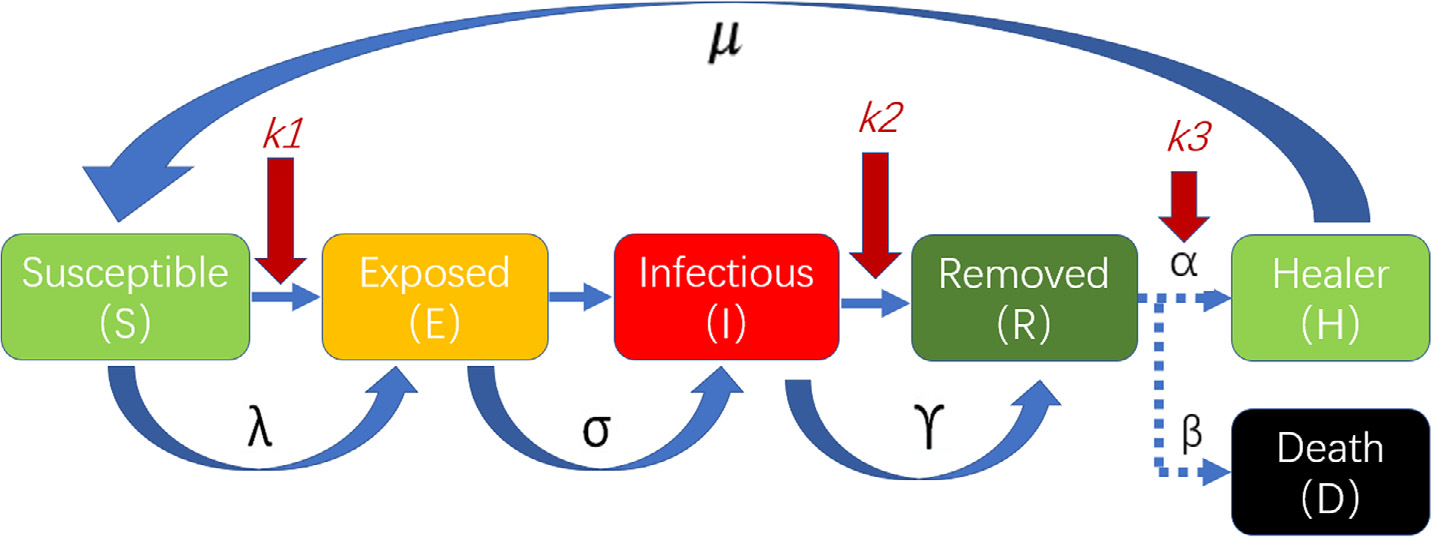
\includegraphics[width=\linewidth]{kseirscheme.png}
	\caption{Schemat działania modelu  \textit {K-SEIR}}
\end{figure}

Teoretyczny model K-SEIR został przekształcony w prosty oprogramowanie, zaimplementowane w języku PYTHON, przy użyciu inżynierii oprogramowania. W szczególności, ukończono zadania związane z projektowaniem interfejsu graficznego użytkownika, logiką sterowania, logiką operacji, kontrolą precyzji, kontrolą prędkości, wizualizacją danych, importem i eksportem danych, dopasowaniem parametrów, wyświetlaniem kluczowych danych oraz innymi konkretnymi treściami.
\newpage
\section{\textbf{Modele agentowe}}

Modele agentowe stanowią komputerowe symulacje, w których agenci, reprezentujący różne jednostki, mogą wejść w interakcję między sobą. Agentami mogą być jednostki takie jak osoby, organizacje, a nawet obszary geograficzne, takie jak województwa czy kraje. Wzajemne oddziaływania między agentami są określone przez zdefiniowane zasady programowe. Każdy z agentów podejmuje decyzje indywidualnie, co może obejmować zarówno proste wybory, na przykład decyzję o kierunku ruchu, jak i bardziej złożone decyzje, takie jak znalezienie konkretnego innego agenta lub sekwencję zdarzeń. W kontekście symulacji zarażeń, tego typu podejście pozwala na realistyczne uwzględnienie nieprzewidywalnych decyzji, jakie może podjąć jednostka.

Jednym z artykułów naukowych, poruszających temat modelowania agentowego pod tytułem: \textit{,,An open-data-driven agent-based model to simulate infectious disease outbreaks''} \cite{bib:artykul1} dostarczy nam cennych informacji na  temat implementacji takich rozwiązań. 

W artykule możemy przeczytać szczegółowe informacje na temat tego co badacze wzięli po uwagę podczas tworzenia swojego modelu.
był on oparty o dane populacji, umiejscowienia szkół i miejsc pracy a także danych dotyczących szczepień. Rzeczywiste dane są używane do określenia struktury wiekowej i płciowej naszych populacji, wraz z właściwym rozkładem wielkości gospodarstw domowych oraz innymi cechami takimi jak wiek dzieci. Następnie dane opisujące lokalizację szkół oraz miejsc pracy dają możliwość wiernego odwzorowania interakcji pomiędzy ludźmi. Na koniec aby ocenić podatność populacji na rozprzestrzenianie się choroby uwzględniono ilość szczepień (badanie opierało się na badaniu epidemii odry).
Następnym krokiem badaczy było wybranie testowanego obszaru i podzielenie go na mniejsze jednostki, w których przebywający ludzie są uznawani za mający kontakt ze sobą. Później należało rozmieścić agentów w odpowiednich domach według danych o populacji. Na koniec należało uwzględnić dodatkowe czynniki między innymi transport. 
Ostatnim krokiem było matematyczne opisane szans na zarażeniem, w tym celu autorzy wykorzystali równanie:

\begin{center}
$R_0 = cpd$
\end{center}

gdzie:\\
$R_0$ - prawdopodobieństwo infekcji. \\
$c$ - liczba kontaktów na jednostkę czasu. \\
$p$ - szansa na zarażenie podczas kontaktu. \\
$d$ - długość trwania infekcji \\

Poprzez przekształcenie równania otrzymano: 
\begin{center}
$ p = \frac{R_0}{cd} $
\end{center}

Dodatkowo w scenariuszach testowych, w których brano pod uwagę szczepienia użyto dodatkowego równania. Jest ono oparte na odporność zbiorowej jednak zmodyfikowane aby uwzględniać skuteczność szczepionki:

\begin{center}
	$V_c = \frac{(1-\frac{1}{R_0})}{V_e}$
\end{center}

gdzie:\\
$V_c$ - objęcie szczepieniami populacji \\
$V_e$ - skuteczność szczepionki. \\

Badacze przetestowali swój program na wielu miastach w Irlandii, ze względu na dostępne dane co do ich struktury oraz populacji.
Dodatkowo model został porównany z rzeczywistymi danych dotyczącymi epidemii odry w Schull, Irlandia w 2012 roku. Ze względu na losowość w modelu efekty każdej z symulacji było nieco inne. 

cyt. \textit{,, (...) Średnia liczba zainfekowanych agentów w różnych próbach wyniosła 17, przy maksymalnej liczbie 90 zainfekowanych agentów w jednym przypadku. Dwadzieścia pięć procent prób skończyło się wybuchem, w którym więcej niż 30 agentów zostało zainfekowanych. Wyniki pokazują, że chociaż średnia dla wszystkich prób jest niższa niż liczba zainfekowanych w przypadku wybuchu w Schull, to liczba faktycznie zainfekowanych osób znajduje się w 75. centylu wyników modelu.'' (...)}\cite{bib:artykul1}

Podsumowując, przewagą modeli agentowych nad modelami takimi jak SEIR jest uwzględnienie decyzji jednostki, przykładowo jeżeli mimo choroby osoba zdecyduje się pójść do szkoły lub pracy, ilość zarażeń wzrośnie lub odwrotnie jeżeli zdecyduje się zostać w domu, ilość zarażeń zmaleje, takie niuanse są wychwytywane dzięki skupieniu się na jednostce. Niestety takie podejście dużo gorzej radzi sobie w miarę zwiększania populacji, dlatego idealnie nadają się do symulacja epidemii w małych miastach ale nie w obrębie całego kraju lub świata.

\section{\textbf{Inne modele symulacji zarażeń}}

Ta część zwróci uwagę na dwie innowacyjne metody modelowania zarażeń, które stanowią wyjątkowe podejście w szerokim spektrum dostępnych metod. Ze względu na obecności różnorodnych podejść do modelowania zarażeń, skoncentrujemy się teraz na dwóch szczególnie interesujących metodach. Pierwszą z nich jest ambitny projekt symulacyjny oparty na algorytmach równoległych, korzystający z obszernych danych dotyczących populacji w Stanach Zjednoczonych. Drugą, szczególnie oryginalną, jest aplikacja wykorzystująca technologię rozszerzonej rzeczywistości do wizualizacji, jak wirus może utrzymywać się na różnych powierzchniach i w konsekwencji jak może się szerzyć. Przechodząc do analizy tych dwóch wyjątkowych podejść w celu zidentyfikowania ich specyficznych zalet.

\subsection{\textbf{EpiSimdemics - równoległy algorytm symulacji epidemii}}
\textit{,,EpiSimdemics: an efficient algorithm for simulating the spread of infectious disease over large realistic social networks''} \cite{bib:konferencja} Jest bardzo ambitnym projektem wykorzystującym do obliczeń równoległy algorytm do symulowania rozprzestrzeniania się zarażeń w dużych i realistycznych symulowanych społeczeństwach. Badacze postanowili zasymulować niemalże statystycznie nierozróżnialną populację Stanów Zjednoczonych. Każdy z agentów w symulacji jest inny i opisany przez nawet do 163 zmiennych demograficznych z spisu ludności. Algorytm \textit{EpiSimdemics} opiera się na:
\begin{itemize}
	\item kolekcji jednostek z wartościami stanu i lokalnych reguł przejść między stanami
	\item grafie interakcji przechwytującego lokalną zależność jednostki od swoich sąsiednich jednostek
	\item sekwencji aktualizacji lub harmonogramu, takiego że związek przyczynowo-skutkowy w systemie jest 	reprezentowany przez składanie lokalnych odwzorowań
\end{itemize}
Z tych założeń są formułowane równania przejść stanów dla każdego z osobników w symulacji. Reprezentujące w jaki sposób stan wierzchołka (osobnika) i jego sąsiadujących wierzchołków będzie zmieniał się w trakcie trwania programu. Innymi słowy definiuje proces rozprzestrzeniania się choroby w siatce wierzchołków reprezentujących społeczeństwo.
	Dzięki zastosowaniu tak skomplikowanego systemu, program \textit{EpiSimdemics} posiada zdolność dostarczania szczegółowych informacji na temat rozprzestrzeniania się choroby w populacji, obejmujących takie detale jak konkretny zestaw osób zainfekowanych, miejsce zarażenia oraz kto ich zarażał.
\subsection{\textbf{Zastosowanie rozszerzonej rzeczywistości w symulacji zarażeń}}

Zainspirowani globalną pandemią COVID-19, badacze postanowili stworzyć innowacyjną aplikację pokazującą rozprzestrzenianie się wirusa poprzez różnego rodzaju powierzchnie i przedmioty, z którymi stykamy się w codziennym życiu. Udało się to dzięki wykorzystaniu rozszerzonej rzeczywistości, co pozwoliło na dokładne zobrazowanie, jak wirusy i bakterie mogą pozostawać na tych powierzchniach oraz jak łatwo mogą być przenoszone poprzez kontakty ręczne i inne interakcje. Aplikacja umożliwia użytkownikowi stworzenie własnego patogenu lub wybranie istniejącego, a następnie korzystając z kamery pozwala umieścić go w świecie wirtualnym. Użytkownik może śledzić, jak długo patogen utrzymuje się w danym miejscu, potencjalnie stanowiąc ryzyko przeniesienia się na inną osobę. Swoje spostrzeżenia i wnioski zawarli w artykule \textit{Bio-Virus Spread Simulation in Real 3D Space using Augmented Reality}\cite{bib:artykul2}

\begin{figure}[h!]
	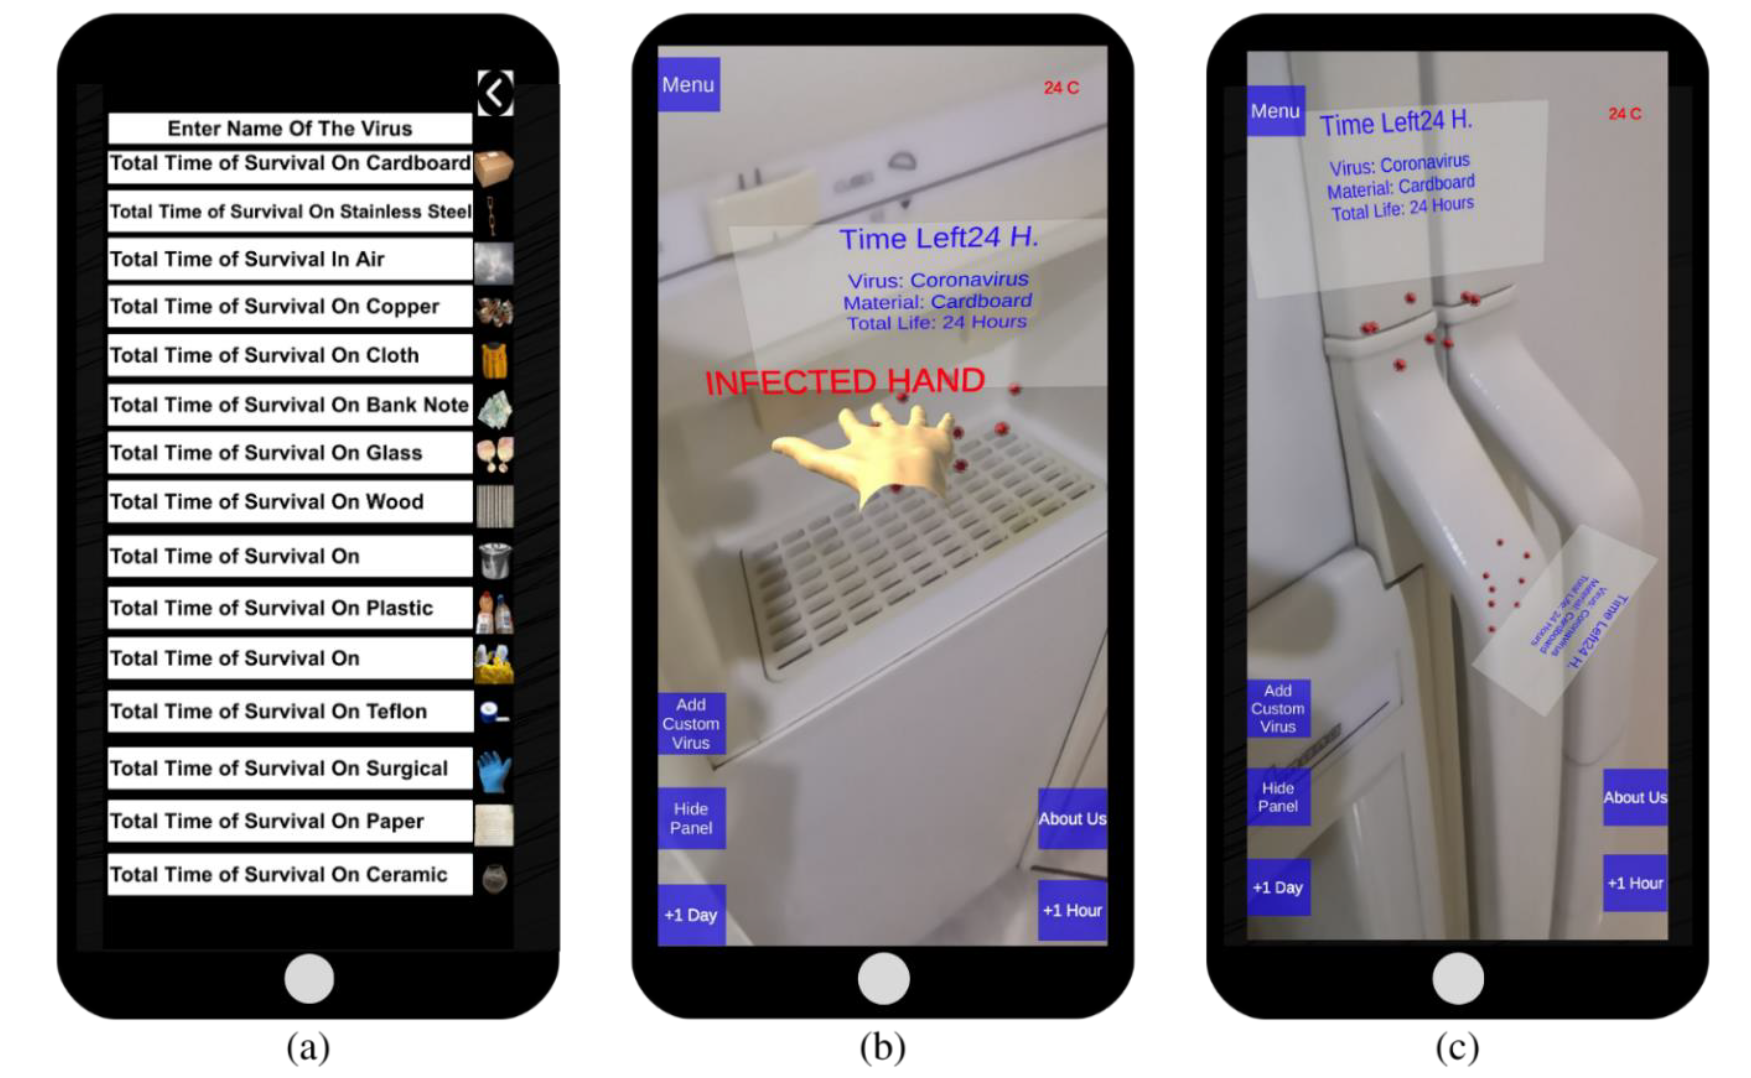
\includegraphics[width=\linewidth]{VirusIn3DSpaces.png}
	\caption{Demonstracja działania aplikacji: (a) dostosowywanie niestandardowego wirusa, (b) wprowadzenie wirusa w rzeczywistego świata, (c) wirus widoczny w rozszerzonej rzeczywistości z panelem informacyjnym.}
\end{figure}
%%%%%%%%%%%%%%%%%%%%%%%%



 % analiza tematu

% TODO
\chapter{Wymagania i narzędzia}
\label{ch:wymagania-i-narzedzia}
%\begin{itemize}
%	\item wymagania funkcjonalne i niefunkcjonalne
%	\item przypadki użycia (diagramy UML) -- dla prac, w których mają zastosowanie
%	\item opis narzędzi, metod eksperymentalnych, metod modelowania itp.
%	\item metodyka pracy nad projektowaniem i implementacją -- dla prac, w których ma to zastosowanie
%\end{itemize}
Rozdział omawia kluczowe aspekty dotyczące aplikacji do symulowania rozprzestrzeniania się zarażeń o nazwie \textit{InfektoSym}. Rozpocznie się od analizy i przedstawienia wymagań funkcjonalnych oraz niefunkcjonalnych. Następnie przybliży technologie wykorzystane w aplikacji. Dodatkowo, dokładnie wyjaśni działanie zaimplementowanego modelu symulacji rozprzestrzeniania się choroby, a także w jaki sposób aplikacja oddziałuje z użytkownikiem i jakie rezultaty może dostarczyć. Ten rozdział stanowi istotne wprowadzenie do zrozumienia zarówno technicznego, jak i funkcjonalnego aspektu projektu.

\section{\textbf{Wymagania funkcjonalne i niefunkcjonalne}}

Skoncentrowano się na opracowaniu symulacji, ze szczególnym naciskiem na środowisko wewnątrz budynków. Taka decyzja wynika z faktu, że ludzie spędzają większość swojego czasu w budynkach, a duże zagęszczenie populacji w takich miejscach stwarza optymalne warunki dla rozprzestrzeniania się chorób.

\subsection{\textbf{Wymagania funkcjonalne}}
\begin{itemize}
	\item \textbf{ Symulacja ruchu i interakcji:}
	
	Aplikacja pozwala na śledzenie ruchu każdej postaci w biurze w czasie rzeczywistym.
	Interakcje pomiędzy postaciami są symulowane z uwzględnieniem różnych scenariuszy, takich jak rozmowy, wspólna praca, czy przerwy.
	W momencie, gdy jedna postać zostaje zarażona, aplikacja monitoruje, czy i jak szybko choroba rozprzestrzenia się na inne postacie poprzez ich bezpośrednie kontakty.
	\item \textbf{Wizualizacja stanów zdrowia:}
	
	Na ekranie widoczne są dynamiczne wskaźniki zdrowia każdej postaci, pozwalające użytkownikowi śledzić ich aktualny stan (zdrowy, narażony, zarażony).
	Symulacja obejmuje także wizualizację okresów inkubacji oraz wyzdrowienia, umożliwiając obserwację zmian stanów zdrowia w czasie rzeczywistym.
	\item \textbf{Monitorowanie kontaktów i narażenia:}
	
	Aplikacja zbiera dane dotyczące kontaktów pomiędzy postaciami, identyfikując te, które mogą prowadzić do potencjalnego zarażenia.
	Wizualizacja narażeń obejmuje różne aspekty, takie jak dystans, czas trwania kontaktu oraz ewentualne zastosowane środki ochrony osobistej.
	\item \textbf{Wariacje scenariuszy:}
	
	Aplikacja umożliwia eksperymentowanie z różnymi scenariuszami zarażenia poprzez dostosowanie parametrów symulacji. Użytkownik może modyfikować takie czynniki jak dystans zarażenia, czas do zarażenia, czy skuteczność maseczek, co pozwala na badanie wpływu tych parametrów na proces rozprzestrzeniania się infekcji w przestrzeni biurowej.

	\item \textbf{Wysoce parametryzowalna symulacja:}
	\begin{enumerate}
		\item \textbf{Dystans zarażenia:}
		
		Użytkownik ma możliwość określenia maksymalnego dystansu, na jakim wirus może się przenosić między agentami.
		\item \textbf{Czas do zarażenia:}
		
		Określenie czasu, jaki musi upłynąć w bliskim kontakcie z zarażoną postacią, aby doszło do zarażenia.
		\item \textbf{Zaraźliwość Patogenu:}
		
		Parametr definiujący zdolność wirusa do zarażania innych postaci w danym środowisku symulacyjnym.
		\item \textbf{Średni okres inkubacji:}
		
		Ustalenie czasu, jaki upływa od momentu zarażenia do pojawienia się objawów u zarażonej postaci.
		\item \textbf{Procent Populacji Noszący Maseczki:}
		
		Możliwość określenia odsetka populacji, który stosuje środki ochrony osobistej w postaci noszenia maseczek.
		\item \textbf{Skuteczność maseczek:}
		
		Parametr określający, o ile procent zmniejsza się dystans zarażenia dla osób noszących maseczki.
		\item \textbf{Liczebność populacji:}
		
		Określenie ogólnej liczby postaci uczestniczących w symulacji.
		
		\item \textbf{Początkowy Procent Zarażonych:}
		
		Określenie procentowej liczby zarażonych w początkowej populacji.
		\item \textbf{Odporność populacji:}
		
		Ustalenie procentowej naturalnej odporność na wirusa.
		\item \textbf{Długość Symulacji:}
		
		Określenie czasu trwania symulacji w jednostkach czasu.
		\item \textbf{Prędkość Symulacji:}
		
		Umożliwienie regulacji prędkości symulacji, włączając przyspieszenie do 100-krotności normalnej prędkości.
		
		\item \textbf{Średni czas wykrycia:}
		
		Ustalenie czasu, jaki upływa od momentu pojawienia się objawów, do ich wykrycia i zlecenia kwarantanny.
		\item \textbf{Pauzowanie Symulacji:}
		
		Dodatkowa funkcjonalność, która pozwala na zatrzymywanie symulacji w dowolnym momencie i jej późniejsze wznowienie.
	\end{enumerate}
\end{itemize}
\subsection{\textbf{Wymagania niefunkcjonalne}}
\begin{itemize}
	\item\textbf{  Intuicyjny interfejs:}
	
	Interfejs użytkownika powinien być zaprojektowany w sposób intuicyjny, umożliwiając łatwe poruszanie się po aplikacji i korzystanie z jej funkcji. Elementy graficzne, przyciski i opcje powinny być jasne i zrozumiałe dla użytkownika końcowego.
	\item\textbf{ Stabilność:}
	
	Aplikacja powinna charakteryzować się stabilnością działania, eliminując nieoczekiwane błędy, które mogą prowadzić do awarii. Wszystkie funkcje aplikacji powinny działać zgodnie z oczekiwaniami, zapewniając płynne doświadczenie użytkownika.
	\item\textbf{ Odporność na awarie:}
	
	Aplikacja powinna być odporna na awarie poprzez implementację mechanizmów zabezpieczających, takich jak obsługa błędów, przywracanie stanu aplikacji po awarii, oraz minimalizacja wpływu awarii na całość systemu.
	
	\item \textbf{Płynność symulacji:}
	
	Aplikacja powinna zapewniać płynną symulację nawet przy dużej ilości agentów uczestniczących w scenariuszu. Optymalizacje i zoptymalizowany kod powinny umożliwiać utrzymanie odpowiedniej prędkości symulacji, niezależnie od skomplikowania scenariusza.
	
	\item\textbf{ Responsywność interfejsu:}
	
	Interfejs użytkownika powinien reagować szybko na akcje użytkownika, zapewniając natychmiastowe odpowiedzi na interakcje, co przyczyni się do lepszego doświadczenia użytkownika.
\end{itemize}
\section{\textbf{Wybrana technologia}}

Rozważając wybór technologii do stworzenia aplikacji \textit{InfektoSym}, zdecydowano się na silnik gier Unity. Wybór ten był podyktowany kilkoma kluczowymi czynnikami, mającymi istotne znaczenie dla skuteczności i efektywności projektu.

Przede wszystkim, istnienie dużej społeczności użytkowników stanowiło istotny argument. Unity cieszy się uznaniem ze względu na szeroki dostęp do materiałów szkoleniowych wideo, aktywność na forum dyskusyjnych oraz obfite źródła dokumentacji online. Ta społeczność stanowi nie tylko źródło wsparcia, lecz także umożliwia szybsze rozwiązywanie potencjalnych problemów napotkanych podczas procesu tworzenia aplikacji.

Duże możliwości rozwoju były kolejnym czynnikiem decydującym o wyborze Unity. Silnik ten oferuje elastyczność i skalowalność, co pozwala na rozbudowę aplikacji w miarę ewentualnych zmian w wymaganiach projektu.

Aspekt wydajności miał kluczowe znaczenie dla płynności symulacji. Unity, dzięki zoptymalizowanym mechanizmom renderowania i obsługi fizyki, pierwotnie zaprojektowanych do tworzenia gier komputerowych, świetnie odnajduje się w przeprowadzaniu wszelkiego rodzaju symulacji gdzie ważna jest reprezentacja graficzna.

Gotowe narzędzia dostarczane przez Unity, takie jak edytory interfejsu użytkownika czy wbudowany system nawigacji dla poruszających się obiektów, znacząco skracają czas potrzebny na rozwój aplikacji. To ułatwienie pozwala skupić się na kluczowych aspektach projektu.

Podsumowując, wybór Unity jako platformy do tworzenia \textit{InfektoSym} wynikał z korzyści płynących z bogatego ekosystemu, wydajności silnika oraz dostępności narzędzi ułatwiających pracę, co zapewniło efektywny i skuteczny proces realizacji projektu.
\section{\textbf{Model symulacji rozprzestrzeniania się zarażeń zastosowany w InfektoSym}}

Model symulacji zaimplementowany w \textit{InfektoSym} stanowi połączenie modelu SEIR z podejściem opartym na agentach, mając na celu dokładne odwzorowanie rozprzestrzeniania się zarażeń. Struktura modelu zakłada podział populacji na cztery główne grupy, analogiczne do SEIR:
\begin{itemize}
	\item \textbf{Zdrowi (Susceptible)}  - grupa osób zdrowych.
	\item \textbf{Narażeni (Exposed)} - grupa osób, które miały kontakt z zarażonym i są potencjalnie podatne na zakażenie.
	\item \textbf{Zarażeni (Infected)} - grupa osób, u których choroba jest aktywna, co stanowi źródło dalszego zarażania.
	\item \textbf{Usunięci (Removed)} - osoby, które zostały zidentyfikowane jako chore i zostały odizolowane.
\end{itemize}
Symulacja opiera się na podejściu agentowym, skupiając uwagę na indywidualnych decyzjach każdego z osobników. Ten szczególny nacisk na indywidualność umożliwia uchwycenie subtelności wprowadzanych przez decyzje jednostki, co jest istotne dla precyzyjnego modelowania dynamiki rozprzestrzeniania się zarażeń.

\subsection{\textbf{Równania opisujące model symulacji}}
Założenia modelu oraz parametry symulacji pozwalają wyizolować równania opisujące prawdopodobieństwo zarażenia w określonych warunkach.

Przejście agenta ze stanu zdrowego do narażonego obliczane jest według następujących parametrów i równań:

Jeżeli zdrowa osoba przebywa w odległości $x < d_{maks}$, gdzie $x$ to odległość od zarażonego, a $d$ to maksymalny dystans, na jaki patogen może się przenosić w czasie $t_k > t_z$, gdzie $t_k$ to czas kontaktu, a $t_z$ to minimalny czas potrzebny do zakażenia. Szansa na przeniesienie do grupy narażonych (exposed) określana jest przez parametr zdolności zarażania patogenu $R_0$ (jeżeli $R_0 = 50$, przy każdym kontakcie szansa na narażenie wynosi 50\%).
Dodatkowymi parametrami grającymi tu rolę jest posiadanie maseczki i jej skuteczność. Dystans przenoszenia się patogenu jest procentowo zmniejszany w zależności od ustawionej skuteczności maseczek.\\

Kiedy agent zostanie uznany za narażonego, program wylicza procentowe szanse na rozwój choroby. Na podstawie wzoru:

\begin{center}
	$P_z = R_0 \cdot (1 - I)$
\end{center}

gdzie:\\
$P_z \in <0,100> $ - szansa na zostanie zarażonym, wyrażona w \% \\
$R_0 \in <0,100>$ - współczynnik zakażalności patogenu \\
$I \in <0,1>$ - odporność jednostki.\\

Wykonywane jest losowanie; jeżeli tak, osobnik zostanie przeniesiony do grupy zarażonych (Infected), jeżeli nie, wróci do puli zdrowych (Susceptible). W obu przypadkach stanie się to po czasie $T_{inkubacji} \pm 24$ godziny (czasu symulacji).

Osoba zakażona jest usuwana z symulacji po czasie $T_{wykrycia} \pm 24$ godziny (czasu symulacji).

\begin{figure}[h!]
	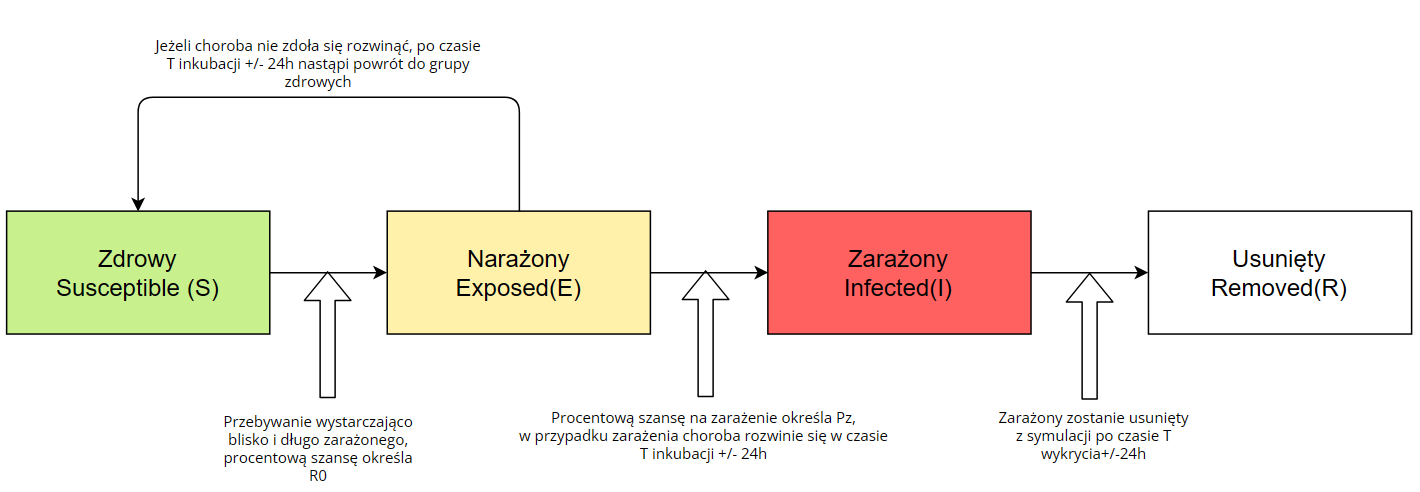
\includegraphics[width=\linewidth]{diagramModelu.png}
	\caption{Schemat działania modelu użytego w \textit{InfektoSym}}
\end{figure}

\subsection{\textbf{Symulacja zachowań ludzkich}}
W ramach symulacji zachowań ludzkich w aplikacji, agenci mają zdefiniowane konkretne czynności, które mogą wykonywać. Poniżej przedstawiono proces realizacji tych aktywności (poniższe wartości czasowe odnoszą się do czasu symulacji):

\begin{itemize}
	\item \textbf{Początkowe losowanie:}
	\begin{itemize}
		\item Agent pojawiając się w symulacji, losuje jedną z czterech podstawowych akcji:\textit{ losowe spacerowanie, praca, przerwa} lub \textit{lunch}.
		\item Każda akcja(oprócz losowego spacerowania) trwa od 1 do 4 godzin.
	\end{itemize}
	
	\item \textbf{Zmiana akcji:}
	\begin{itemize}
		\item Po zakończeniu aktualnej akcji, agent wybiera nową spośród \textit{ losowego spacerowania, pracy, przerwy} lub \textit{lunchu}.
		\item Ten proces powtarza się, co pozwala agentowi na cykliczne zmiany działań.
	\end{itemize}
	
	\item \textbf{Rozmowy:}
	\begin{itemize}
		\item Kiedy agenci się mijają, mają 1\% szansy na rozpoczęcie rozmowy.
		\item Rozmowa trwa od 10 minut do 1 godziny, a po jej zakończeniu agent wybiera nową akcję.
	\end{itemize}
	
	\item \textbf{Praca, odpoczynek i lunch:}
	\begin{itemize}
		\item Jeśli agent zdecyduje się pracować, odpoczywać lub coś zjeść sprawdza dostępność odpowiednio biurek, miejsc na kanapie, stolików w kuchni.
		\item Siada przy pierwszym wolnym miejscu i wykonuje czynność od 1 do 4 godzin, po czym wybiera nową akcję.
		\item W przypadku braku wolnych miejsc agent rozpoczyna \textit{ losowe spacerowanie}.
	\end{itemize}
\end{itemize}

Ten proces symulacyjny pozwala na odwzorowanie różnorodnych działań agentów, obejmujących pracę, odpoczynek, jedzenie i społeczne interakcje. Losowanie czasu trwania i zmiana akcji wprowadza naturalność w zachowaniach agentów.



 % Wymagania i narzędzia

% TODO
\chapter{Specyfikacja zewnętrzna}
\label{ch:04}

Aplikacja została stworzona w środowisku Unity i zapewnia interaktywną symulację rozprzestrzeniania się zarażeń w przestrzeni biurowej. Pozwala na zmianę wielu parametrów wpływających na przebieg symulacji. Ma na celu w prosty i zrozumiały dla każdego sposób pokazywać rozprzestrzenianie się choroby. Przeznaczona jest głównie dla użytkowników korzystających z komputerów osobistych z systemem operacyjnym Windows.

\section{Wymagania}

Sprzęt i oprogramowanie potrzebne do uruchomienia aplikacji:
\begin{itemize}
	\item Komputer z systemem operacyjnym Windows.
	\item Ekran o rozdzielczości co najmniej 1280x720 pikseli.
	\item Karta graficzna wspierająca OpenGL 3.2 lub nowszy.
	\item System operacyjny: Windows 7/8/10 i nowsze.
	\item Zainstalowany runtime Unity w wersji zgodnej z aplikacją.
\end{itemize}

\section{Uruchamianie aplikacji}

Aby skorzystać z aplikacji, należy wykonać poniższe kroki:

\begin{enumerate}
	\item Pobrać instalator aplikacji.
	\item Uruchomić instalator.
	\item Postępować zgodnie z instrukcjami aż do zakończenia instalacji.
	\item Uruchomić aplikację dwukrotnie klikając jej skrót lub plik wykonwalny \textit{exe} znajdujący się w folderze instalacji.
\end{enumerate}

\section{Obsługa aplikacji}

Do obsługi aplikacji wystarczy myszka, która umożliwia interakcję z interfejsem graficznym. Aplikacja nie wymaga dodatkowego sprzętu.
\begin{itemize}
	\item \textbf{Wizualizacja}\\
	Graficzne przedstawienie symulacji znajduje się po lewej stronie okna aplikacji. Mapa biura, odzwierciedla przestrzeń do pracy, kuchnię oraz miejsce wypoczynku. Szczegółowy opis mapy i jej poszczególnych elementów znajduje się na rysunku \ref{fig:simMap}.

	\begin{figure}[h!]
		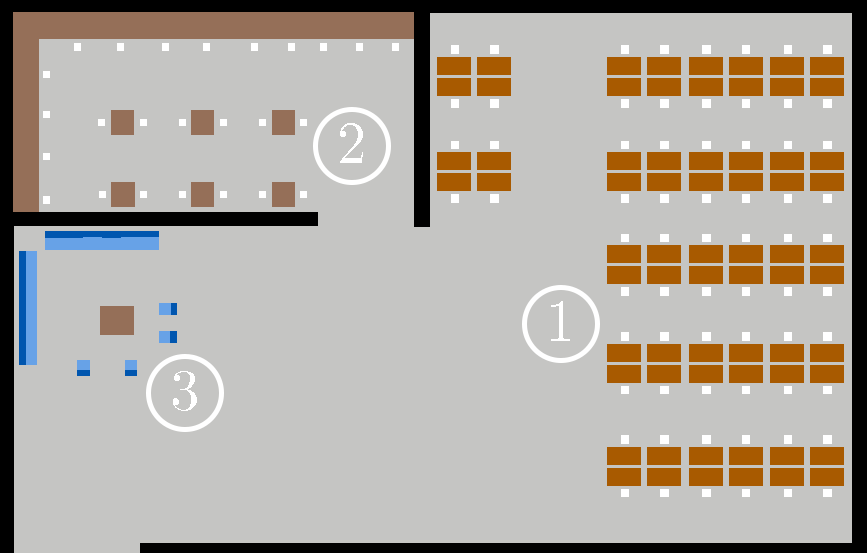
\includegraphics[width=\linewidth]{mapWithNumbers.png}
		\caption{Mapa biura: 1. Biurka do pracy, 2. Kuchnia ze stolikami, 3. Miejsce wypoczynku}
		\label{fig:simMap}
	\end{figure}
	
	\item \textbf{Ustawianie Parametrów Symulacji}
	
	Dostosowywanie parametrów odbywa się poprzez ustawianie suwaków znajdujących się z prawej strony (widocznych na rysunku \ref{fig:runningSim} przy numerze pierwszym) za pomocą myszki. Parametry należy ustawić przed rozpoczęciem symulacji, ich zmiana w jej trakcie nie wpłynie na jej przebieg, a nowe ustawienia zostaną wprowadzone dopiero po restarcie symulacji. Wyjątkiem jest prędkość symulacji, którą można zmieniać w trakcie działania programu.\\
	\textbf{Lista dostępnych parametrów:}
	\begin{itemize}
		\item \textbf{Dystans zarażenia:}\\
		 Dystans przenoszenia się wirusa.
		
		\item \textbf{Czas do zarażenia:}\\
		 Czas(minuty) bliskiego kontaktu z chorym, aby doszło do zarażenia.

		\item \textbf{Zaraźliwość patogenu:}\\
		 Zdolność wirusa do zarażania.
		
		\item \textbf{Średni okres inkubacji:}\\
		 Czas(dni) od narażenia do rozwinięcia się objawów.

		\item \textbf{Procent populacji noszący maseczki:}\\
		Procentowa ilość ludzi noszących maseczki.

		\item \textbf{Skuteczność maseczek:}\\
		Określa jak bardzo skuteczne są maseczki w ograniczaniu zasięgu wirusa.
		
		\item \textbf{Liczebność populacji:}\\
		Ogólna liczba postaci uczestniczących w symulacji.
		
		\item \textbf{Początkowy procent zarażonych:}\\
		Procentowa liczba zarażonych na początku symulacji.
		
		\item \textbf{Odporność populacji:}\\
		Odporności osobników na zarażenie.

		\item \textbf{Długość symulacji:}\\
		Ilość dni trwania symulacji.
		
		\item \textbf{Prędkość symulacji:}\\
		Umożliwienie regulacji prędkości symulacji, włączając przyspieszenie do 100-krotności normalnej prędkości.
		
		\item \textbf{Średni czas wykrycia:}\\
		Czas(dni) jaki upływa od momentu pojawienia się objawów do ich wykrycia i zlecenia kwarantanny.
	\end{itemize}
	
	\item \textbf{Rozpoczęcie symulacji i jej kontrola}\\
	Do kontroli symulacji służą przyciski widoczne na rysunku \ref{fig:runningSim} przy numerze drugim. Są to \textit{Start}, \textit{Pauza} i \textit{Restart}. 
	
	\begin{itemize}
	\item \textbf{Start}\\
	Uruchamia symulację lub ją wznawia.
	
	\item \textbf{Pauza}\\
	Zatrzymuje symulacje. Po jej wznowieniu parametry symulacji, pozycje agentów i czas się nie zmieniają.
	
	\item \textbf{Restart}\\
	Kończy symulację. Usuwa wszystkich agentów, po uruchomieniu symulacji agenci zostaną stworzeni na nowo wraz ze zaktualizowanymi parametrami.
	\end{itemize}

	\begin{figure}[h!]
		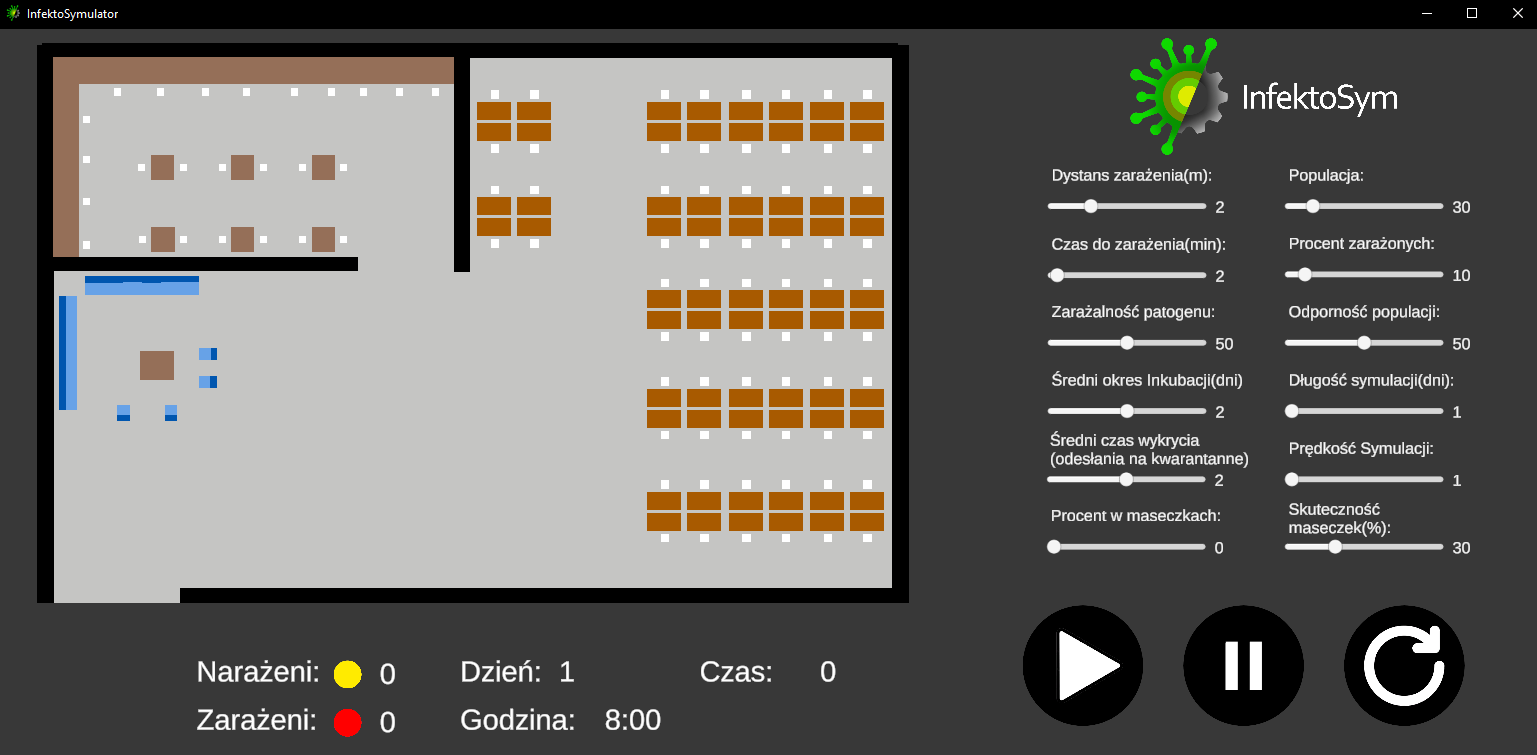
\includegraphics[width=\linewidth]{beforeSim.png}
		\caption{Ekran początkowy aplikacji.}
		\label{fig:beforeSim}
	\end{figure}
	
	\item \textbf{Zakończenie symulacji}\\
	Użytkownik może zakończyć symulację w każdej chwili klikając w przycisk \textit{Restart}. W przeciwnym przypadku symulacja zakończy się automatycznie po ustawionym na początku czasie jej trwania oraz zostanie wyświetlony ekran z podsumowaniem widoczny na rysunku \ref{fig:endSim}.
	
	\item \textbf{Statystyki symulacji}\\
	Podczas trwania symulacji możliwe jest bieżące monitorowanie jej statystyk, co widać na rysunku \ref{fig:beforeSim} przy numerze trzecim. Są to: liczba osób narażonych, liczba zarażonych, aktualny czas w środowisku symulacyjnym oraz rzeczywisty czas od rozpoczęcia.
	
	\begin{figure}[h!]
		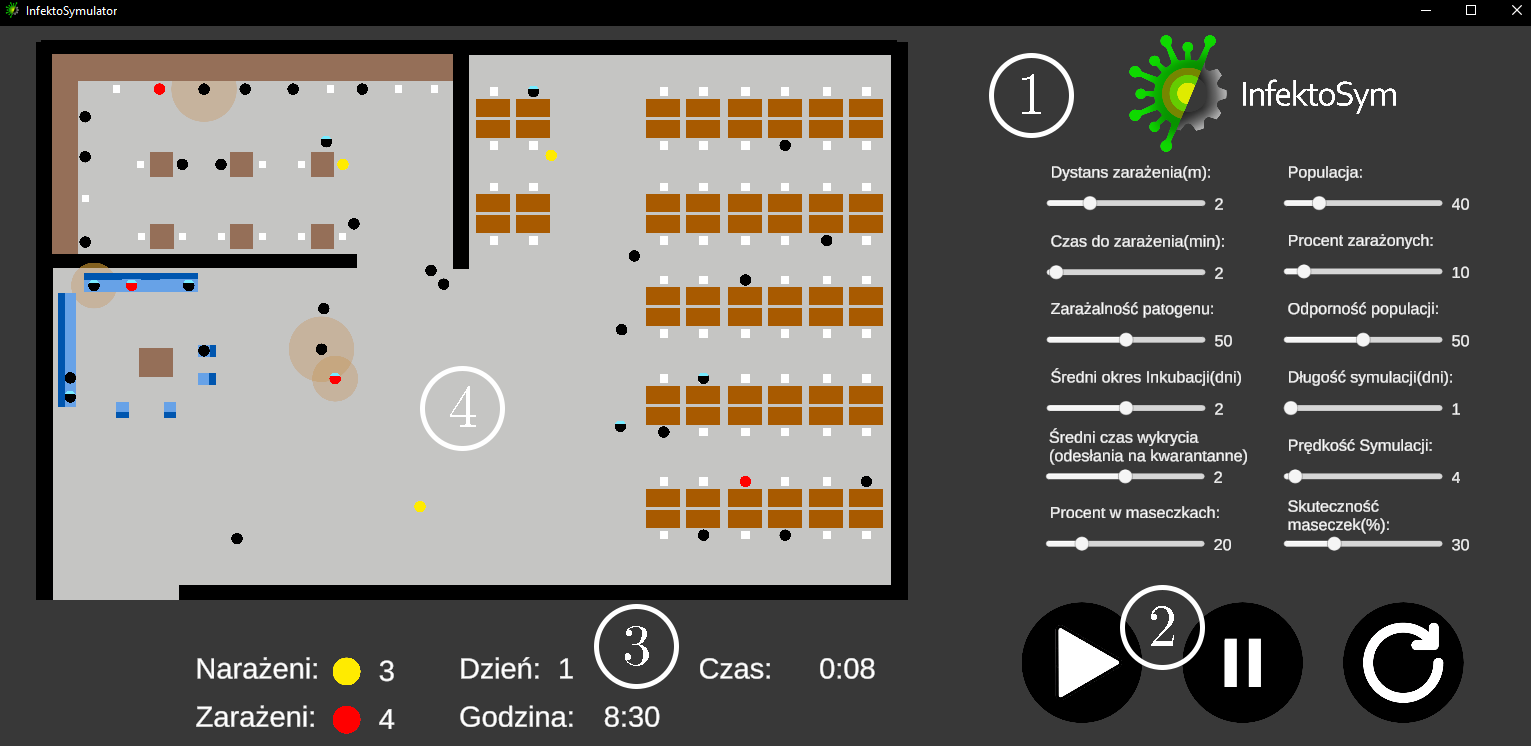
\includegraphics[width=\linewidth]{runningSimwithNumbers.png}
		\caption{Ekran podczas działającej symulacji: 1. Suwaki do ustawiania parametrów, 2. Przyciski kontrolujące 3. Aktualne statystyki i czas, 4. Wizualizacja}
		\label{fig:runningSim}
	\end{figure}
	
	\begin{figure}[h!]
		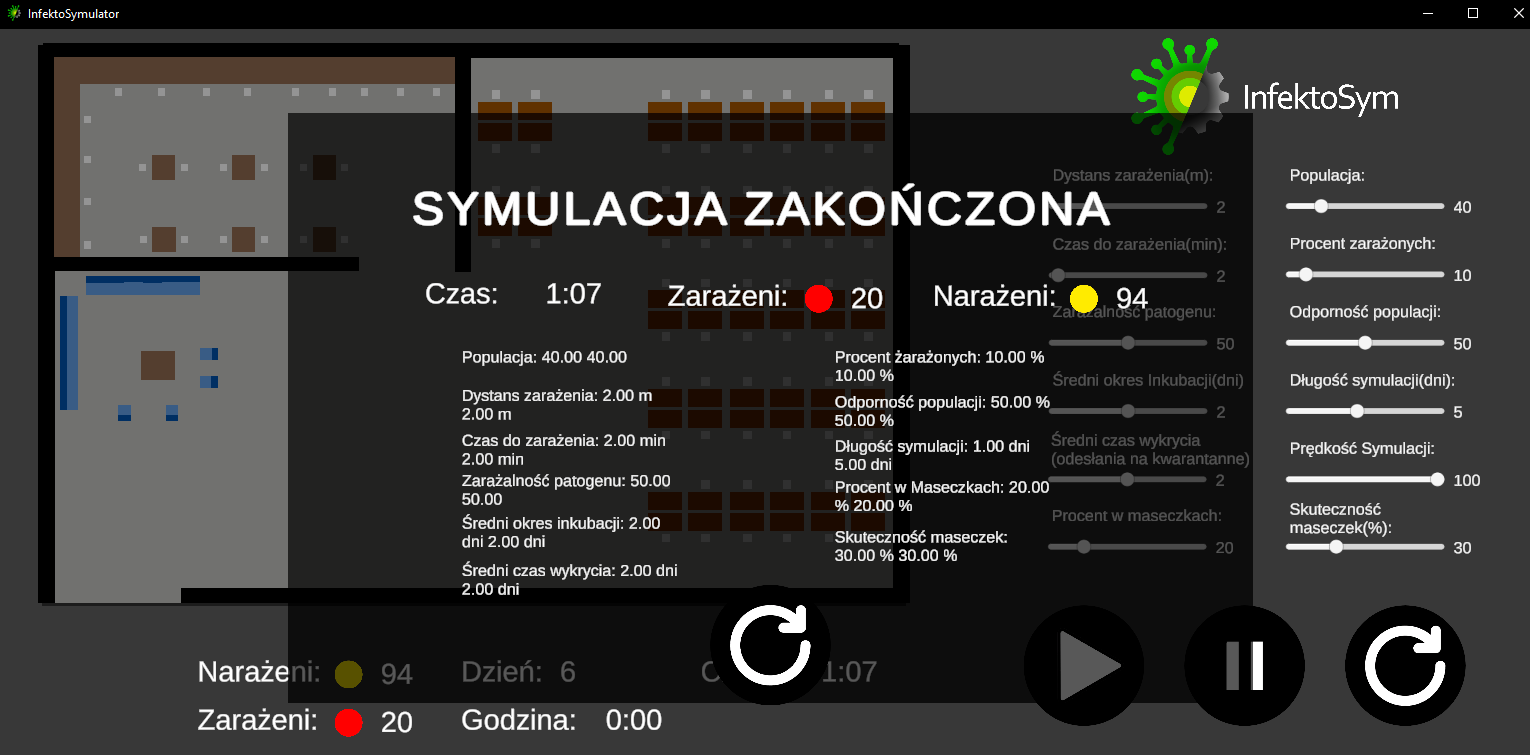
\includegraphics[width=\linewidth]{endSim.png}
		\caption{Ekran zakończenia symulacji}
		\label{fig:endSim}
	\end{figure}
\end{itemize}


%%%%%%%%%%%%%%%%%%%%%
%% RYSUNEK Z PLIKU
%
%\begin{figure}
%\centering
%
\includegraphics[width=0.5\textwidth]{./graf/politechnika_sl_logo_bw_pion_pl.pdf}
%\caption{Podpis rysunku zawsze pod rysunkiem.}
%\label{fig:etykieta-rysunku}
%\end{figure}
%Rys. \ref{fig:etykieta-rysunku} przestawia …
%%%%%%%%%%%%%%%%%%%%%
%
%%%%%%%%%%%%%%%%%%%%%
%% WIELE RYSUNKÓW 
%
%\begin{figure}
%\centering
%\begin{subfigure}{0.4\textwidth}
%    
\includegraphics[width=\textwidth]{./graf/politechnika_sl_logo_bw_pion_pl.pdf}
%    \caption{Lewy górny rysunek.}
%    \label{fig:lewy-gorny}
%\end{subfigure}
%\hfill
%\begin{subfigure}{0.4\textwidth}
%    
\includegraphics[width=\textwidth]{./graf/politechnika_sl_logo_bw_pion_pl.pdf}
%    \caption{Prawy górny rysunek.}
%    \label{fig:prawy-gorny}
%\end{subfigure}
%
%\begin{subfigure}{0.4\textwidth}
%    
\includegraphics[width=\textwidth]{./graf/politechnika_sl_logo_bw_pion_pl.pdf}
%    \caption{Lewy dolny rysunek.}
%    \label{fig:lewy-dolny}
%\end{subfigure}
%\hfill
%\begin{subfigure}{0.4\textwidth}
%    
\includegraphics[width=\textwidth]{./graf/politechnika_sl_logo_bw_pion_pl.pdf}
%    \caption{Prawy dolny rysunek.}
%    \label{fig:prawy-dolny}
%\end{subfigure}
%        
%\caption{Wspólny podpis kilku rysunków.}
%\label{fig:wiele-rysunkow}
%\end{figure}
%Rys. \ref{fig:wiele-rysunkow} przestawia wiele ważnych informacji, np. rys. \ref{fig:prawy-gorny} jest na prawo u góry.
%%%%%%%%%%%%%%%%%%%%%


 % [Właściwy dla kierunku -- np. Specyfikacja zewnętrzna]

% TODO
\chapter{Specyfikacja wewnętrzna}
\label{ch:05}

% % % % % % % % % % % % % % % % % % % % % % % % % % % % % % % % % % % 
% Pakiet minted wymaga importu: \usepackage{minted}                 %
% i specjalnego kompilowania:                                       %
% pdflatex -shell-escape main                                       %
% % % % % % % % % % % % % % % % % % % % % % % % % % % % % % % % % % % 
W niniejszym rozdziale Specyfikacji Wewnętrznej dokładnie omówione zostaną kluczowe elementy związane z implementacją projektu. Zaprezentowana będzie architektura systemu, opisane zostaną użyte biblioteki i moduły, przedstawione zastosowane algorytmy, a także zamieszczone zostaną diagramy sekwencyjne, fragmenty kodu oraz idea, która kierowała procesem tworzenia aplikacji. Celem tego rozdziału jest szczegółowe przybliżenie struktury wewnętrznej projektu, zrozumienie jego komponentów oraz logiki działania.

%\section{\textbf{Przedstawienie idei}}
%
%Aplikacja Infektosym jest narzędziem symulacyjnym, które zostało stworzone z myślą o zrozumieniu i analizie rozprzestrzeniania się zarażeń w przestrzeni biurowej. Głównym celem projektu jest dostarczenie interaktywnej platformy umożliwiającej obserwację, analizę oraz testowanie scenariuszy związanych z potencjalnymi wirusowymi infekcjami w środowisku pracy.
%
%\begin{itemize}
%	\item \textbf{Cele Projektu:}
%	\begin{itemize}
%		\item Zapewnienie realistycznego modelu symulacji, uwzględniającego codzienne zachowania ludzkie w biurze.
%		\item Możliwość dostosowywania parametrów symulacji, takich jak dystans zarażenia, czas do zarażenia czy skuteczność maseczek.
%		\item Wizualizacja procesu rozprzestrzeniania się patogenów w czasie rzeczywistym.
%	\end{itemize}
%	\item \textbf{Koncepcje i Założenia:}
%	\begin{itemize}
%		\item Implementacja agentowego podejścia, gdzie każdy osobnik w symulacji podejmuje indywidualne decyzje i reaguje na otoczenie.
%		\item Duża parametryzacja symulacji, umożliwiająca dostosowanie scenariuszy do różnych warunków i kontekstów.
%	\end{itemize}
%	\item \textbf{Kierunki Rozwoju:}
%	\begin{itemize}
%		\item Wprowadzenie zaawansowanych funkcji interakcji między agentami, uwzględniających bardziej złożone scenariusze zachowań.
%		\item Integracja z danymi epidemiologicznymi dla bardziej precyzyjnych analiz i prognoz.
%		\item Dalsza optymalizacja interfejsu użytkownika i dostępność na różnych platformach.
%		\item Wprowadzenie innych scenariuszy np. Szpital, Osiedle, Centrum Handlowe.
%	\end{itemize}
%\end{itemize}

\section{\textbf{Architektura systemu}}

Architektura systemu aplikacji opiera się na modularnym podejściu, skupiającym się na kilku kluczowych skryptach odpowiedzialnych za różne aspekty symulacji.

\begin{itemize}
	\item \textbf{InterfaceScript:}
	\begin{itemize}
		\item Odpowiada za interakcję z użytkownikiem, umożliwiając mu dostosowywanie parametrów symulacji za pomocą sliderów.
		\item Obsługuje przyciski kontroli, takie jak start, pauza, restart, co zapewnia płynną kontrolę nad symulacją.
		\item Wyświetla istotne statystyki dotyczące aktualnego stanu symulacji, umożliwiając użytkownikowi bieżącą analizę danych.
	\end{itemize}
	
	\item \textbf{GlobalClockScript:}
	\begin{itemize}
		\item Pełni rolę zegara w aplikacji, monitorując czas zarówno w skali symulacji, jak i rzeczywistości.
		\item Liczy dni, godziny oraz ilość godzin symulacji od jej rozpoczęcia, co pozwala na śledzenie postępu w czasie.
		\item Zapewnia synchronizację między symulacją a realnym czasem, co jest istotne dla precyzyjnego odwzorowania dynamiki zarażeń.
	\end{itemize}
	
	\item \textbf{HumanSpawner:}
	\begin{itemize}
		\item Inicjalizuje agentów (ludzi) na mapie, ustawiając je zgodnie z parametrami otrzymanymi od InterfaceScript podczas rozpoczęcia symulacji.
		\item Zapewnia jednolite warunki startowe dla agentów, co umożliwia kontrolowaną analizę scenariuszy symulacyjnych.
	\end{itemize}
	
	\item \textbf{HumanScript:}
	\begin{itemize}
		\item Stanowi rdzeń symulacji zachowań ludzkich, przypisany do każdego obiektu reprezentującego osobę na mapie.
		\item Monitoruje kolizje i stosuje algorytmy określające, czy dany osobnik powinien być narażony na ryzyko zarażenia czy też jest już zainfekowany.
		\item Umożliwia kompleksową symulację interakcji między ludźmi i symulowanie ich zachowań.
	\end{itemize}
	
	\item \textbf{SeatScript:}
	\begin{itemize}
		\item Prosty skrypt odpowiedzialny za zarządzanie miejscami siedzącymi, informując, czy dane miejsce jest zajęte czy wolne.
	\end{itemize}
	\item \textbf{GameOverScript:}
	\begin{itemize}
		\item Prosty skrypt odpowiedzialny pokazanie ekranu końcowego z odpowiednimi wynikami i parametrami symulacji.
	\end{itemize}
\end{itemize}

\subsection{Biblioteki i moduły}
Aplikacja została napisana w Unity, wykorzystując standardowe biblioteki i moduły dostępne w tym środowisku. Dodatkowo, do realizacji funkcjonalności związanych z nawigacją postaci została użyta biblioteka Navmesh 2D. Navmesh to technika używana w grach do generowania trójwymiarowych lub dwuwymiarowych map nawigacyjnych, pozwalających postaciom na inteligentne poruszanie się w przestrzeni, omijanie przeszkód i podejmowanie decyzji dotyczących ruchu.

\section{\textbf{Algorytmy}}

W projekcie występuje kilka algorytmów kontrolujących symulację, zajmujących się kontrolą czasu, cyklem dnia i nocy, symulacją przenoszenia się choroby oraz symulacją ludzkich zachowań. Poniżej przedstawiono opis dwóch kluczowych algorytmów:
\subsection{Kontrola rozprzestrzeniania się choroby}
Algorytm ten skupia się na precyzyjnej symulacji interakcji między osobami. W przypadku kolizji między dwiema postaciami jeśli jedna z postaci jest zarażona, mierzy się czas rozpoczęcia i zakończenia kontaktu. Jeżeli ten czas spełnia warunki minimalnego czasu zarażenia, oblicza się szansę na zarażenie zgodnie z zarażalnością wirusa. W przypadku braku narażenia status pozostaje bez zmian. W sytuacji narażenia, status zmienia się na EXPOSED, a następnie oblicza się szansę na rozwinięcie choroby. Jeśli choroba się nie rozwija, status zostaje zmieniony na "healthy". W przypadku rozwinięcia choroby, status zmienia się na INFECTED. W obydwu przypadkach zmiana statusu ma miejsce po określonym czasie inkubacji ($\pm$ 24h). Zarażona osoba zostaje usunięta z symulacji po wykryciu (± 24h). Algorytm przedstawiony jest na diagramie sekwencyjnym \ref{diagramZarazanie}. Implementację algorytmu przedstawiają fragmenty kodu \ref{fig:kod:OnTriggerEnter} i \ref{fig:kod:OnTriggerExit}, dotyczą one zachowania przy rozpoczęciu i zakończeniu kontaktu, przyglądając się funkcji \textit{OnTriggerExit()} możemy zauważyć że to ona jest odpowiedzialna za zmianę statusu osobnika na EXPOSED oraz wywołanie kolejnej funkcji odpowiedzialnej za wyliczenie szansy na rozwinięcie się choroby \ref{fig:kod:CalculateInfection}.

\begin{figure}[h!]
	\centering
	\includegraphics[width=0.6\linewidth]{DiagramKontaktu.png}
	\caption{Sekwencyjny diagram algorytmu kontaktu miedzy agentami}
	\label{diagramZarazanie}
\end{figure}

\subsection{Symulacja zachowań ludzkich}
Ten algorytm odpowiada za symulację codziennych działań ludzi w biurze. Losuje on różne akcje, takie jak \textit{spacerowanie, lunch, przerwa} czy \textit{praca}. W przypadku akcji \textit{praca, lunch} lub \textit{przerwa}, algorytm znajduje dostępne miejsce siedzące i zajmuje je na losowy czas od 1 do 4 godzin, po czym zmienia akcję na kolejną. Jeżeli nie ma wolnego miejsca, akcja zostaje natychmiastowo zmieniona na losowe spacerowanie. W trakcie tych działań, w przypadku spotkania dwóch postaci, istnieje 1\% szansa na rozpoczęcie rozmowy. Po zakończonej rozmowie losowana jest kolejna akcja. Algorytm przedstawiony jest na diagramie sekwencyjnym \ref{diagramZachowanie}. Implementację pokazuje fragment kodu \ref{fig:kod:Activity}, zawiera dwie funkcje kontrolujące rozpoczęcie i zakończenie akcji. Do symulacji konwersacji miedzy agentami wykorzystano analogiczne bardzo podobne rozwiązanie, rozszerzone o dodatkowe kroki konieczne dla tego zachowania.

\begin{figure}[h!]
	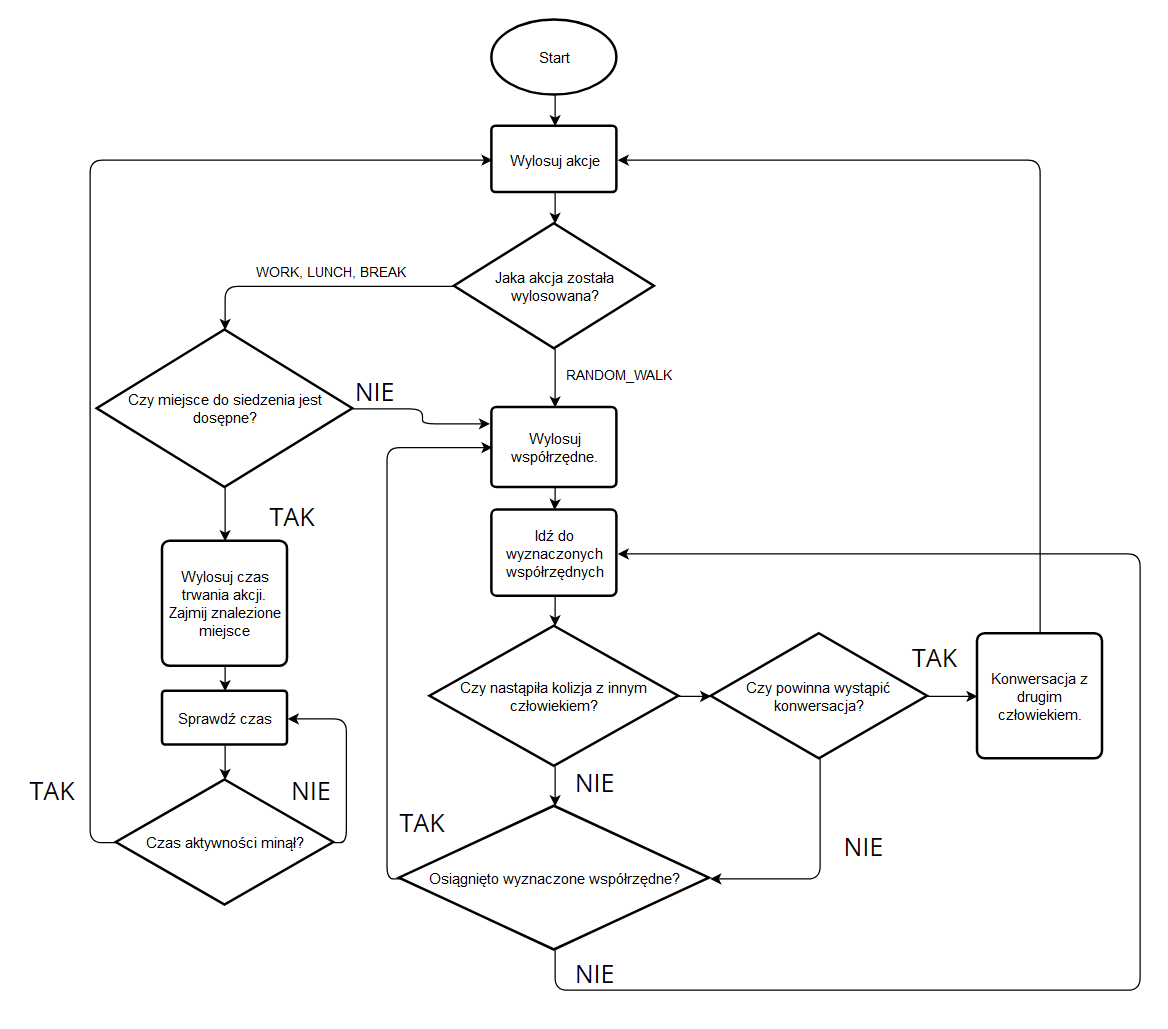
\includegraphics[width=\linewidth]{DiagramAlgorytmuZachowania.png}
	\caption{Sekwencyjny diagram algorytmu symulacji zachowań ludzkich}
	\label{diagramZachowanie}
\end{figure}


%Krótka wstawka kodu w linii tekstu jest możliwa, np.  \lstinline|int a;| (biblioteka \texttt{listings})% lub  \mintinline{C++}|int a;| (biblioteka \texttt{minted})
%. 
%Dłuższe fragmenty lepiej jest umieszczać jako rysunek, np. kod na rys \ref{fig:pseudokod:listings}% i rys. \ref{fig:pseudokod:minted}
%, a naprawdę długie fragmenty – w załączniku.


%\begin{figure}
%\centering
%\begin{lstlisting}
%class test : public basic
%{
%    public:
%      test (int a);
%      friend std::ostream operator<<(std::ostream & s, 
%                                     const test & t);
%    protected:
%      int _a;  
%     
%};
%\end{lstlisting}
%\caption{Pseudokod w \texttt{listings}.}
%\label{fig:pseudokod:listings}
%\end{figure}

%\begin{figure}
%\centering
%\begin{minted}[linenos,frame=lines]{c++}
%class test : public basic
%{
%    public:
%      test (int a);
%      friend std::ostream operator<<(std::ostream & s, 
%                                     const test & t);
%    protected:
%      int _a;  
%      
%};
%\end{minted}
%\caption{Pseudokod w \texttt{minted}.}
%\label{fig:pseudokod:minted}
%\end{figure}


 % [Właściwy dla kierunku -- np. Specyfikacja wewnętrzna]

% TODO
\chapter{Weryfikacja i walidacja}
\label{ch:06}
\begin{itemize}
\item sposób testowania w ramach pracy (np. odniesienie do modelu V)
\item organizacja eksperymentów
\item przypadki testowe zakres testowania (pełny/niepełny)
\item wykryte i usunięte błędy
\item opcjonalnie wyniki badań eksperymentalnych
\end{itemize}

W tym rozdziale przedstawione zostaną techniki sprawdzania i potwierdzania poprawności działania aplikacji. W procesie tworzenia oprogramowania istotne jest nie tylko zaplanowanie i implementacja funkcji, ale także dokładne sprawdzenie, czy rezultaty są zgodne z założeniami projektowymi. Weryfikacja koncentruje się na sprawdzeniu, czy projekt spełnia założenia funkcjonalne i techniczne, natomiast walidacja ocenia, czy to, co zostało zaimplementowane, odpowiada rzeczywistym potrzebom użytkowników. W dalszej części tego rozdziału przedstawione zostaną metody, narzędzia i procedury stosowane w procesie weryfikacji i walidacji.\\

\section{Sposoby testowania i organizacja eksperymentów}

W ramach przeprowadzonych testów aplikacji dokonano ręcznego dostosowania parametrów symulacji. Obejmowały one zakres od maksymalnych do minimalnych wartości oraz różne kombinacje pomiędzy nimi. Kluczowe parametry zostały testowane oddzielnie, a przykładowo długość symulacji poddana była analizie, aby ocenić wpływ zwiększenia liczby cykli dnia i nocy na funkcjonalność. Dodatkowo przetestowano różne wartości procentowe dla zarażonych i osób noszących maseczki. Eksperymentowano również z różnymi liczebnościami populacji, aby zrozumieć, jak wpływają one na symulację zachowań ludzkich.

%
% znalezione błedy 
% po pierwszym dniu maski przestają się pokazywać 
% agenci wypadaja z navmesh
% problem z rezerwowanieiem i zwalnianiem miejsc siedzących

 % Weryfikacja i walidacja

% TODO
\chapter*{Podsumowanie i wnioski}
\label{Podsumowanie i wnioski}
Celem pracy było opracowanie aplikacji symulującej rozprzestrzenianie się zarażeń, ze szczególnym uwzględnieniem środowiska biurowego. Projekt zakładał dostarczenie narzędzia umożliwiającego szeroką parametryzację symulacji, realistyczny model symulacyjny, uwzględnienie codziennych zachowań ludzkich w biurze oraz wizualizacje rozwoju epidemii.

Praca nad projektem symulacyjnym \textit{Infektosym} przyniosła satysfakcjonujące wyniki, spełniające niemal wszystkie postawione wymagania funkcjonalne. Pomimo osiągnięcia sukcesu w realizacji większości celów, pojawiły się pewne ograniczenia, szczególnie związane z liczbą populacji. Symulowanie dużej liczby osób w biurze, przekraczającej 100-150, okazało się niepraktyczne, co stanowi obszar do dalszych rozważań.

\begin{itemize}
	\item \textbf{Osiągnięte cele i wymagania} \\
	 W ramach pracy udało się z powodzeniem zrealizować założone cele oraz spełnić postawione wymagania funkcjonalne. Skonstruowany model symulacyjny pozwolił na wierne odwzorowanie procesu rozprzestrzeniania się chorób w środowisku biurowym.
	
	\item \textbf{Ograniczenia i potencjalne rozwinięcia} \\
	 Pojawiły się pewne ograniczenia związane głównie z liczbą symulowanych osób. W celu lepszej skalowalności należałoby rozważyć alternatywne scenariusze lub większe mapy. Dodatkowo, rozbudowa symulacji zachowań ludzkich oraz zwiększenie liczby scenariuszy to obszary, które mogą znacząco wzbogacić funkcjonalność aplikacji.
	
	\item \textbf{Ewentualne kierunki rozwoju} \\
	 Przyszłe prace nad projektem mogłyby skupić się na ulepszaniu symulacji zachowań ludzkich, wprowadzając bardziej złożone scenariusze i interakcje między agentami. Dodatkowo, warto rozważyć rozbudowę funkcjonalności o nowe scenariusze, co umożliwi bardziej wszechstronne testowanie i analizę zachowań w różnych warunkach. Ponadto, istnieje możliwość dodania funkcji zapisywania parametrów i wyników symulacji do pliku, co ułatwiłoby dalszą analizę oraz przechowywanie danych w celu późniejszego wykorzystania.
\end{itemize}

W świetle uzyskanych wyników, projekt \textit{Infektosym} stanowi solidną podstawę do dalszych prac rozwojowych, mających na celu jeszcze bardziej zaawansowane modele symulacyjne i bogatsze doświadczenia użytkowników. 
 % Podsumowanie i wnioski

\backmatter

%\bibliographystyle{plplain}  % bibtex
%\bibliography{biblio/biblio} % bibtex
\printbibliography           % biblatex
\addcontentsline{toc}{chapter}{Bibliografia}

\begin{appendices}

% TODO
\chapter{Spis skrótów i symboli}

\begin{itemize}
\item[SIR] Suceptible, Infected, Removed (podatni-zainfekowani-ozdrowieńcy)
\item[SEIR] Suceptible, Exposed, Infected, Removed (podatni-wystawieni-zainfekowani-ozdrowieńcy)
\item[MVC] model -- widok -- kontroler (ang. \english{model--view--controller}) 
\item[$N$] liczebność zbioru danych
\item[$\mu$] stopnień przyleżności do zbioru
\item[$\mathbb{E}$] zbiór krawędzi grafu
\item[$\mathcal{L}$] transformata Laplace'a 
\end{itemize}
 % Spis skrótów i symboli

% TODO
\chapter{Źródła}
\begin{figure}[!h]
	\begin{lstlisting}
		private void OnTriggerEnter2D(Collider2D collider)
		{
			humanScript otherHuman = collider.GetComponent<humanScript>();
			int conversation = UnityEngine.Random.Range(0,100);
			if (conversation == 1)
			{
				otherHuman.Conversation();
				Conversation();
			}
			if(otherHuman.GetStatus() == Status.INFECTED && status==Status.HEALTHY)
			{
				ShowRange();
				timeEnter = Time.time;
			}
			if(status == Status.INFECTED && otherHuman.GetStatus() == Status.HEALTHY)
			{
				ShowRange();
			}
		}
	\end{lstlisting}
	\caption{Funkcja obsługująca początek kontaktu miedzy agentami.}
	\label{fig:kod:OnTriggerEnter}
\end{figure}


\begin{figure}
	\begin{lstlisting}
		private void OnTriggerExit2D(Collider2D collider)
		{
			humanScript otherHuman = collider.GetComponent<humanScript>();
			if(otherHuman.GetStatus() == Status.INFECTED && status==Status.HEALTHY)
			{
				timeExit = Time.time;
				
				float contactDuration = timeExit - timeEnter;
				
				if (contactDuration > timeToInfection)
				{
					int exposed = UnityEngine.Random.Range(0,100);
					if(exposed < virusSpreadFactor)
					{
						status = Status.EXPOSED;
						body.color = Color.yellow;
						simInterface.IncreaseExposed();
						CalculateInfection();
					}
				}
			}
			HideRange();
		}
	\end{lstlisting}
	\caption{Funkcja obsługująca koniec kontaktu miedzy agentami.}
	\label{fig:kod:OnTriggerExit}
\end{figure}


\begin{figure}
	\begin{lstlisting}
		privatevoid CalculateInfection()
		{
			int infectionProbabilty = (int)(virusSpreadFactor*(1 - immunity));
			int attempt = UnityEngine.Random.Range(1,100);
			if(attempt < infectionProbabilty)
			{
				infectionTime = clock.GetHoursPassed() + UnityEngine.Random.Range(incubationPeriod-24, incubationPeriod+24);
				willBeInfected = true;
			}
			else
			{
				infectionTime = clock.GetHoursPassed() + 24;
				willBeInfected = false;
			}
		}
	\end{lstlisting}
	\caption{Funkcja wyliczająca szansę na rozwinięcie się choroby.}
	\label{fig:kod:CalculateInfection}
\end{figure}

\begin{figure}
	\begin{lstlisting}
		private void StartActivity()
		{
			activity = (Activity)UnityEngine.Random.Range(0,4);
			bool seatFound = false;
			switch(activity)
			{
				case Activity.WORK:
				seatFound = SearchSeat(desks);
				break;
				case Activity.BREAK:
				seatFound = SearchSeat(sofas);
				break;
				case Activity.LUNCH:
				seatFound = SearchSeat(kitchenSeats);
				break;
				default:
				break;
			}
			if(!seatFound)
			{
				activity = Activity.RANDOM_WALK;
			}
		}
		
		private void EndActivity()
		{
			if(currentActivityEndTime < clock.GetHour())
			{
				ReleaseSeat();
				StartActivity();
			}
		}
	\end{lstlisting}
	\caption{Funkcja wyliczająca szansę na rozwinięcie się choroby.}
	\label{fig:kod:Activity}
\end{figure}

% % % % % % % % % % % % % % % % % % % % % % % % % % % % % % % % % % % 
% Pakiet minted wymaga odkomentowania w pliku config/settings.tex   %
% importu pakietu minted: \usepackage{minted}                       %
% i specjalnego kompilowania:                                       %
% pdflatex -shell-escape praca                                      %
% % % % % % % % % % % % % % % % % % % % % % % % % % % % % % % % % % % 

%\begin{minted}[linenos,breaklines,frame=lines]{c++}
%if (_nClusters < 1)
%   throw std::string ("unknown number of clusters");
%if (_nIterations < 1 and _epsilon < 0)
%   throw std::string ("You should set a maximal number of iteration or minimal difference -- epsilon.");
%if (_nIterations > 0 and _epsilon > 0)
%   throw std::string ("Both number of iterations and minimal epsilon set -- you should set either number of iterations or minimal epsilon.");
%\end{minted}
 % Źródła

% TODO
\chapter{Lista dodatkowych plików, uzupełniających tekst pracy} 


W systemie do pracy dołączono dodatkowe pliki zawierające:
\begin{itemize}
\item \textit{InfektoSymulatorSource.zip} - spakowany folder zawierający pliki z kodem źródłowym
\item \textit{infektosym-installer-1.0.exe} - instalator aplikacji \textit{InfektoSym}
\end{itemize}
 % Lista dodatkowych plików, uzupełniających tekst pracy

\listoffigures
\addcontentsline{toc}{chapter}{Spis rysunków}
\listoftables
\addcontentsline{toc}{chapter}{Spis tabel}

\end{appendices}

\end{document}


%% Finis coronat opus.

